%%%%%%%%%%%%%%%%%%%%%%%%%%%%%%%%%%%%%%%%%%%%%%%%%%%%%%%%%%%%%%%%%%%%%%%%%%%%%%
%
% タイトル TeX用テンプレート 
% バージョン 2016-8-23 (Tu) 初版
% 作成者 北山天斗,剱崎健太郎
% 作成場所 金沢工業高等専門学校
% 用途 2段組レポートの作成等
%
%%%%%%%%%%%%%%%%%%%%%%%%%%%%%%%%%%%%%%%%%%%%%%%%%%%%%%%%%%%%%%%%%%%%%%%%%%%%%%%%
\documentclass[a4paper]{jarticle}
\usepackage{sice-si}
\usepackage{amsmath} 
\usepackage[dvipdfmx]{graphicx}

%%%%%%%%%%%%%%%%%%%%%%%%%%%%%%%%%%%%%%%%%%%%%%%%%%%%%%%%%%%%%%%%%%%%%%%%%%%%%%%%
\begin{document}\title{教育用マルチコプターの開発}
\name{北山天斗,剱崎健太郎(金沢工業高等専門学校)}
\etitle{English Title}
\ename{Takato KITAYAMA,Kentro KENZAKI(Kanazawa Technical College)}
\abst{
本研究室では機械の制御について研究を行っている.今年度は近年注目されているマルチコプター(以下ドローン)の研究開発に取り組む.
マルチコプターとは3つ以上のローターを持つ無人航空機である.一般に流通しているものは4つのローターを持つマルチコプター(以下クアッドコプター)である.
ローターが4つであると,前後左右の姿勢制御がイメージしやすい.そのため本研究では4つのローターを持つクアッドコプターの研究開発を行う.
}

\maketitle
%%%%%%%%%%%%%%%%%%%%%%%%%%%%%%%%%%%%%%%%%%%%%%%%%%%%%%%%%%%%%%%%%%%%%%%%%%%%%%%%
\section{はじめに}

\subsection{研究の背景}
近年注目されているドローンであるが,開発に取り組まれているのは屋外向けのものが主である.
例えば大手通販企業amazonではドローンを使った宅配システムなどが開発されている.
また,テレビ番組でもドローンを使用して撮影された映像が時折放送されている.
しかし,ドローンは屋内での使用用途が少ないため屋内向けドローンはあまり注目されていない.
本研究室ではそこに注目し屋内向けドローンの用途を見つけ出し,その研究開発を行う.
また,ドローンのプロペラに巻き込まれて怪我をするという事故が多く見受けられる.
これを未然に防ぐため,機体を覆うものを取り付け安全性の向上を試みる.

\subsection{研究の目的}
前述の理由から屋内においてドローンでできそうなことを挙げ,その目標を達成するために必要なハードウェア,ソフトウェアの開発に取り組む.

本研究室ではつくばチャレンジに向け単眼カメラを用いた三次元復元,マッピングシステムの開発が行われた.
そのシステムの使用にはカメラの移動が必要不可欠である.
ドローンであれば前後左右だけでなく上下にも自由に動くことができるため,このシステムの使用に適している.
そこでドローンにこのシステムを搭載し,指定した始点と終点までの間の3次元マッピングを自動で行うことを目的として研究開発を行う.

\subsection{本論文の構成}
本論文は前半でハードウェア開発,後半でソフトウェア開発について述べる.

%%%%%%%%%%%%%%%%%%%%%%%%%%%%%%%%%%%%%%%%%%%%%%%%%%%%%%%%%%%%%%%%%%%%%%%%%%%%%%%

\section{ハードウェア開発の目標}
ドローン1機の積載重量には限りがある.そのため目的達成に必要なものを搭載すると,ドローン1機では足りなくなる.
そこでドローンの機能を複数機に分割し,分割した複数機のドローンを編隊飛行させる.
また,ドローンのプロペラに巻き込まれて怪我をする事故の防止と落下時の衝撃から本体を保護するためドローンを球体で覆う.
この目標達成のための必要事項を示す.

\subsection{機体の設計製作}
3次元マッピングを行う上で必要な装置の重量を測定したところ,ドローンは3機以上必要であることが判明した.
そのため機体は3機製作する.
アルミ製のアームと樹脂製の取付板,RaspberryPi(以下RPi)とNavio、T-MOTOR製のモーター・ESC・プロペラを用いて機体を設計製作する.

\subsection{球体}
機体の大きさから外径510mm内径450mmとなるように輪状のスチレンボードを組み立てて半球を2つ作り,組み合わせて機体を覆う.
CADで作成した球体のイメージを図\ref{fig:sphere-CAD}に示す.

\begin{figure}[htbp]
 \begin{center}
  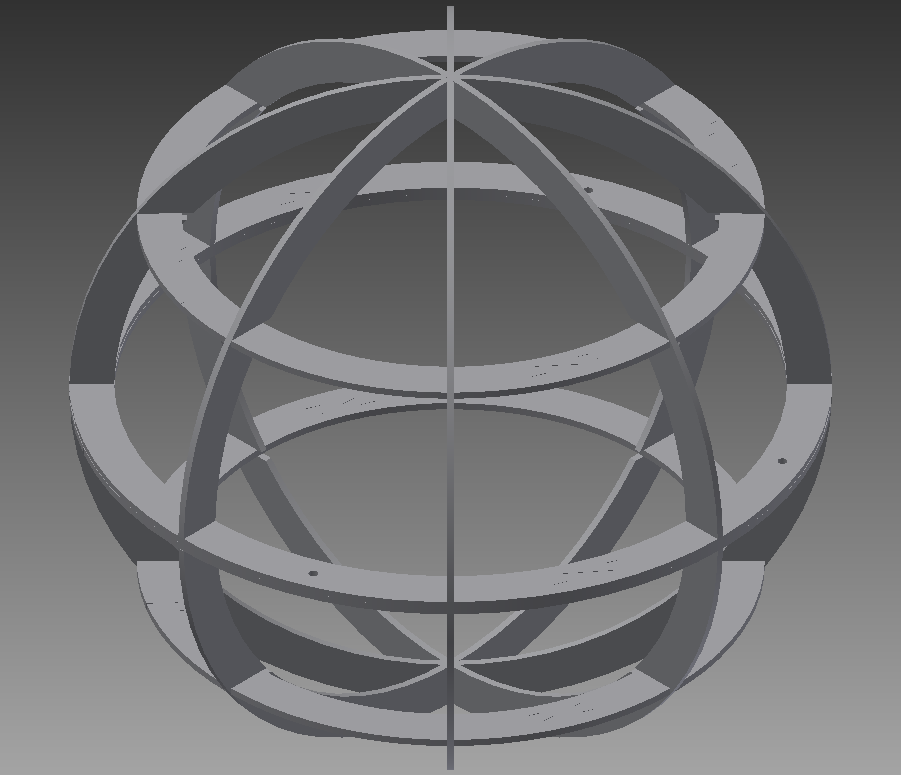
\includegraphics[width=50mm]{image/sphere-CAD.png}
  \caption{球体イメージ}
  \label{fig:sphere-CAD}
 \end{center}
\end{figure}

\section{ハードウェア開発の結果}

\subsection{本体}

\subsubsection{試作1号機}
はじめに試作1号機として,80mm×80mm,厚さ2mmのアルミ角管を高さ20mmに切断し各面にアームを取り付けたものを試作した.
実際に製作した試作1号機を図\ref{fig:drone-1},球体1号機と組み合わせた球体ドローン1号機を図\ref{fig:1}に示す.
また球体と組み合わせた際の重量は750gであった.
この試作1号機では、アームの縦方向の荷重に対する強度やバッテリーなどの取り付け位置・方法が問題となった.

\subsubsection{試作2号機、3号機}
試作1号機での問題点を改良し,試作2号機と3号機を同時に製作した.
アームの縦方向の荷重に対する強度は,25mm×15mm、厚さ1.5mmのアルミ角管を半分に切断したコの字型のものを図\ref{fig:arm}のように交差させたものに変更することで改良した.
バッテリーの取り付け位置・方法は,ABS樹脂板をレーザー加工機で加工することで図\ref{fig:RPi-board}のような専用の取付板を製作して改良を行った.
試作3号機と球体3号機を組み合わせた球体ドローン3号機を\ref{fig:3}に示す.3号機の重量は約716gで1号機と比較して35g程度の軽量化ができた.

\subsubsection{制御実験機}
それまでに製作していた球体2号機,3号機が大破する事案が発生した(後述).
そのため,プログラムによる制御の安定化がある程度実現できるまでの実験機として,制御実験機を製作した.
試作2号機の本体をベースとして各アーム先端と機体中央下部に足を取り付け,最低限の安全性を確保するためプラスチックダンボールの輪を取り付けたメンテナンスが容易なものを製作した.
製作した制御実験機を図\ref{fig:test-machine}に示す.

足があるため離着陸が容易なため,制御実験を行う上では非常に扱いが容易であった.
中央下部にも足を取り付けていたが着地の衝撃が予想以上に強く,アーム中央が沈むように歪んだ.

\subsubsection{本機体1号機}
研究室にあった直径12mmのCFRP(Carbon Fiber Reinforced Plastics:炭素繊維強化プラスチック)のパイプを利用して新しい機体を開発した.
各アームに2本のパイプを使用し,中央で固定用パーツで上下から挟み込んで固定する.
またモーターの取り付け位置等にはパイプ間に板を取り付ける.
アームの材料の違いから軽量化が見込まれていたが,固定パーツが重く全体の重量は増加してしまった.
製作した本機体1号機を図\ref{fig:drone-4}に示す.

\subsection{球体}

\subsubsection{1号機}
輪状のスチレンボードを分割し,スチのりで接着して組み立てた.
製作した球体1号機を図\ref{fig:sphere-1}に示す.
幾度か使用していると接合部のスチレンボードの紙がスチレン材から剥がれてしまった.

\subsubsection{2号機}
1号機の構造ではスチレン材と紙が剥離してしまうので,図\ref{fig:kigumi}のように極力木組み構造で組み立てるように変更した.
製作した球体2号機を図\ref{fig:sphere-2}に示す.

\subsubsection{3号機}
1号機や2号機のように手作業で加工する場合球体1機の製作にとても時間がかかってしまため,スチレンボードの加工をレーザー加工機で行うことにした.
しかし,レーザー加工機で加工する場合,切断面のスチレン材がレーザー光の熱により溶けて凹むことが判明した.
接着のためには広い接着面積が必要なので,接着面以外をレーザー加工機で加工し接着が必要な部分を手作業で加工することにした.
製作した球体3号機を図\ref{fig:sphere-3}に示す.

\subsubsection{4号機}
上記のように3つの球体を製作したが,いずれも試験飛行や体験休学での催しとしてドローンを飛ばしていたところ幾度か墜落を繰り返す内に破損してしまった.
そのため球体の材質や構造などを再検討する必要がある.
新たに製作する球体の材質にはプラスチックダンボールを使用する.
プラスチックダンボールの性質として図\ref{fig:cardboard}のように方向によって強度が違うため,球体の上下部分に最も強度が高い部分を用いるように製作する.
製作した球体4号機を図\ref{fig:sphere-4}に示す.


\section{考察}
以上の結果から重量と強度を考慮すると,CFRPで試作2号機のようなコの字型のアームを交差させた形状を一体成型により製作することが望ましいと考えられる.
球体はプラスチックダンボールで製作したことにより,落下時に最も強度が高い部分が当たるため壊れにくく目的に最も沿ったものとなったと考えられる.


\section{ソフトウェア開発の目標}
目的の達成のためには自律飛行とドローン間の通信制御が必要である.
ドローンの自律飛行にはPID制御を用いて飛行を行い,画像処理による3次元復元と3次元マッピングにより自己位置推定などを行う.
ドローン間の通信にはRPiを無線LANアクセスポイントとして用いることができるため,この機能を利用しての全ドローンを1つのネットワークに接続させて通信を行う.

\subsection{PID制御}
自律飛行を成功させるには,ドローンが安定して飛行できる必要がある.
そのため本研究ではPID制御を用いて飛行を安定化させる.
PIDとは比例(Proportional),積分(Integral),微分(Differential)の英語の頭文字をとったものである.
目標とする値と現在の値の差に比例,積分,微分の制御を行いそれらの要素に補正値ゲインを掛けて足し合わせることにより目標とする値に近づける制御である.

\subsection{コントローラー}
本研究では,最終的には自律飛行を行うが制御が安定するまでの間コントローラーを使用して操作を行いゲインの調整などを行った.
コントローラーにはDUALSHOCK3を用いた.
コントローラーの右スティックをスロットルとヨー方向の制御に割り当て,左スティックをロール方向とピッチ方向の制御に割り当てた.
新しい機能が思いついた場合,使用していないボタンに機能を割り当てることができる.


\section{ソフトウェア開発の結果}

\subsection{自律飛行に至るまで}
自律制御を行う前段階として,DUALSHOCK3をBluetoothでRPiに接続しドローンの操作を行う.
本研究におけるドローンの座標系とモーターの回転方向を示したものを図\ref{fig:dronemotor}に示す.

x,y,z軸それぞれの回転をx軸がロール,y軸がピッチ,z軸がヨーと呼び,それぞれ右ネジの回転方向を正とする.
Navioのセンサから得られる情報から,ロール・ピッチ・ヨー方向のPID制御を行いドローンの動作を制御する.
このPID制御の結果を用いて自律飛行に繋げる.

%\subsection{自律飛行}


\subsection{ドローン間の通信}
RPiの無線LAN機能を使用し,すべてのドローンを1つのネットワークに接続することに成功した.
これにより他の機体の位置などの情報をやりとりする.

\subsection{画像処理プログラムや音声認識プログラム}
同研究室で開発したプログラムを搭載した.
RPiの処理速度が遅いため画像処理プログラムがうまく動作しなかった.
音声認識プログラムはドローンが駆動していない間はうまく動作していたが,ドローンの駆動音がノイズとなりうまく動作しなかった.


\section{考察}
当初の目的だあった自律制御はうまくいったため良かったと考えられる.
画像処理プログラムはRPiでも動作するライト版を開発することが求められる.
音声認識プログラムはノイズの除去機能を別途で開発することが求められる.

\section{おわりに}
ドローンを球体で覆うことにより,今までにない新規性が得られたと考えられる.
また、球体で覆ったことによりドローンのプロペラで人を傷つけるような事故が減り,壁などにぶつかった時ドローン本体が破損しにくくなると考えられる.




\begin{figure*}[b]
 \begin{center}
  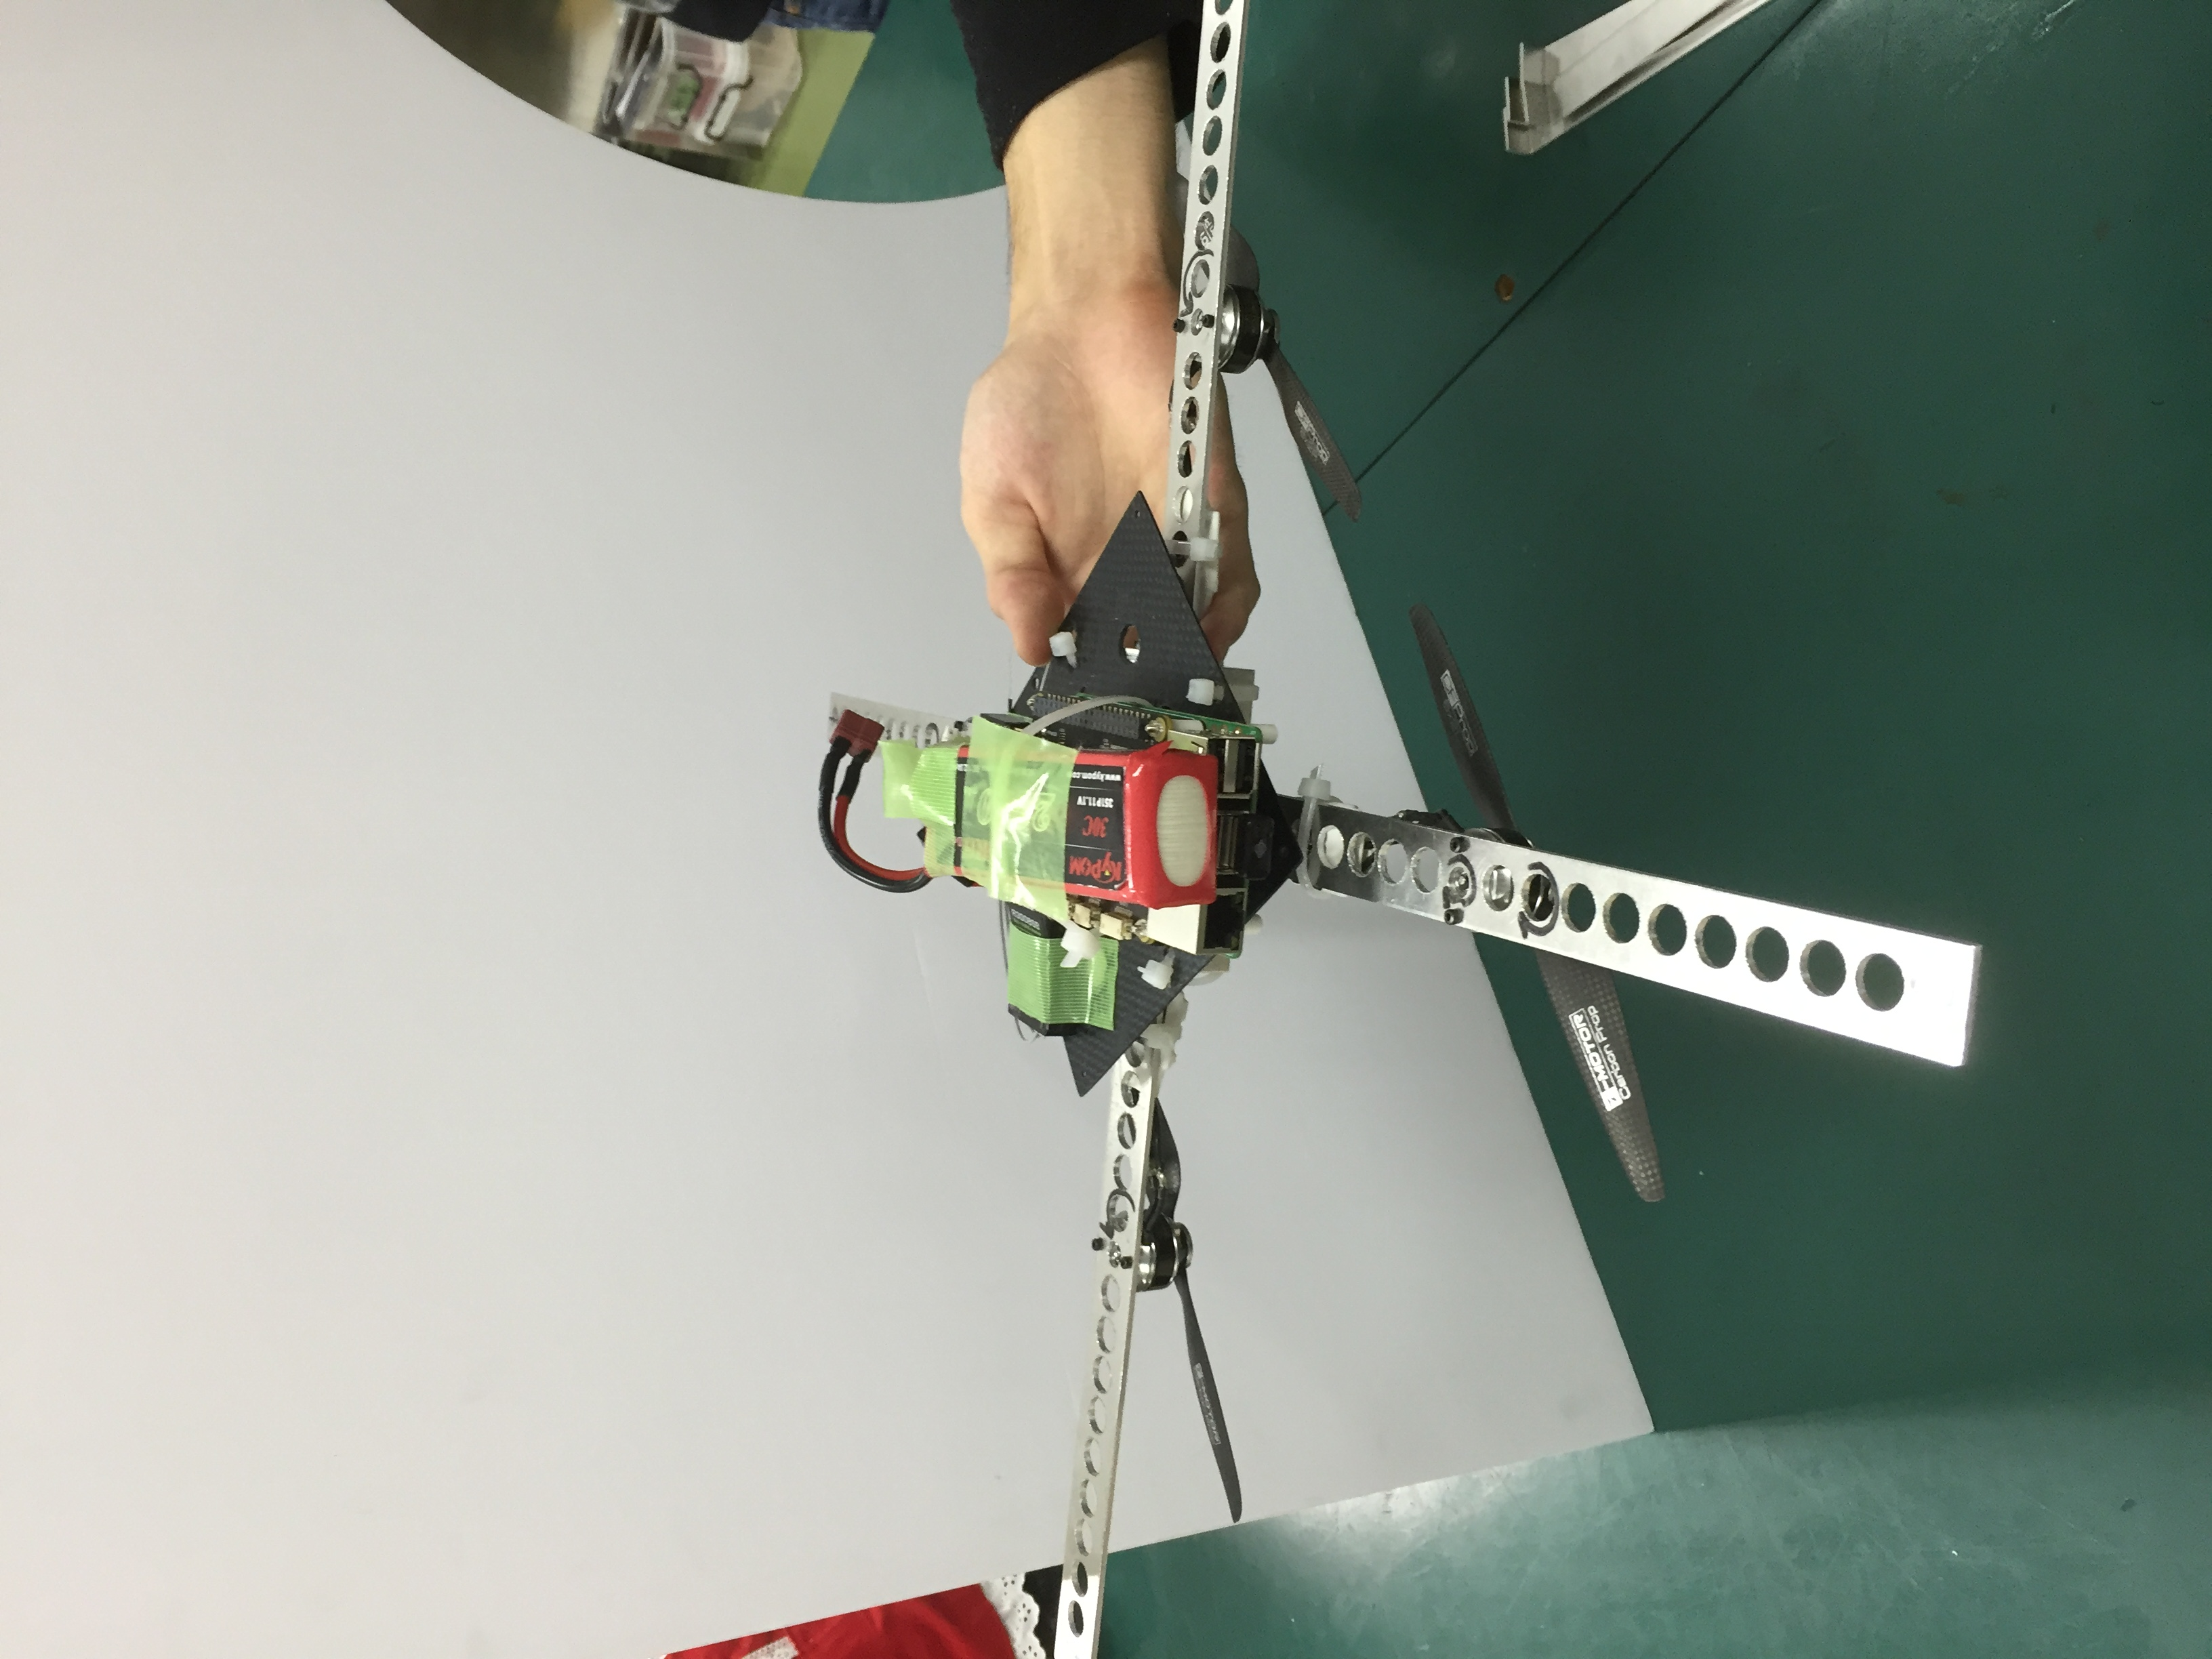
\includegraphics[width=50mm]{image/drone-1.JPG}
  \caption{試作機1号機}
  \label{fig:drone-1}
 \end{center}
\end{figure*}

\begin{figure*}[b]
 \begin{center}
  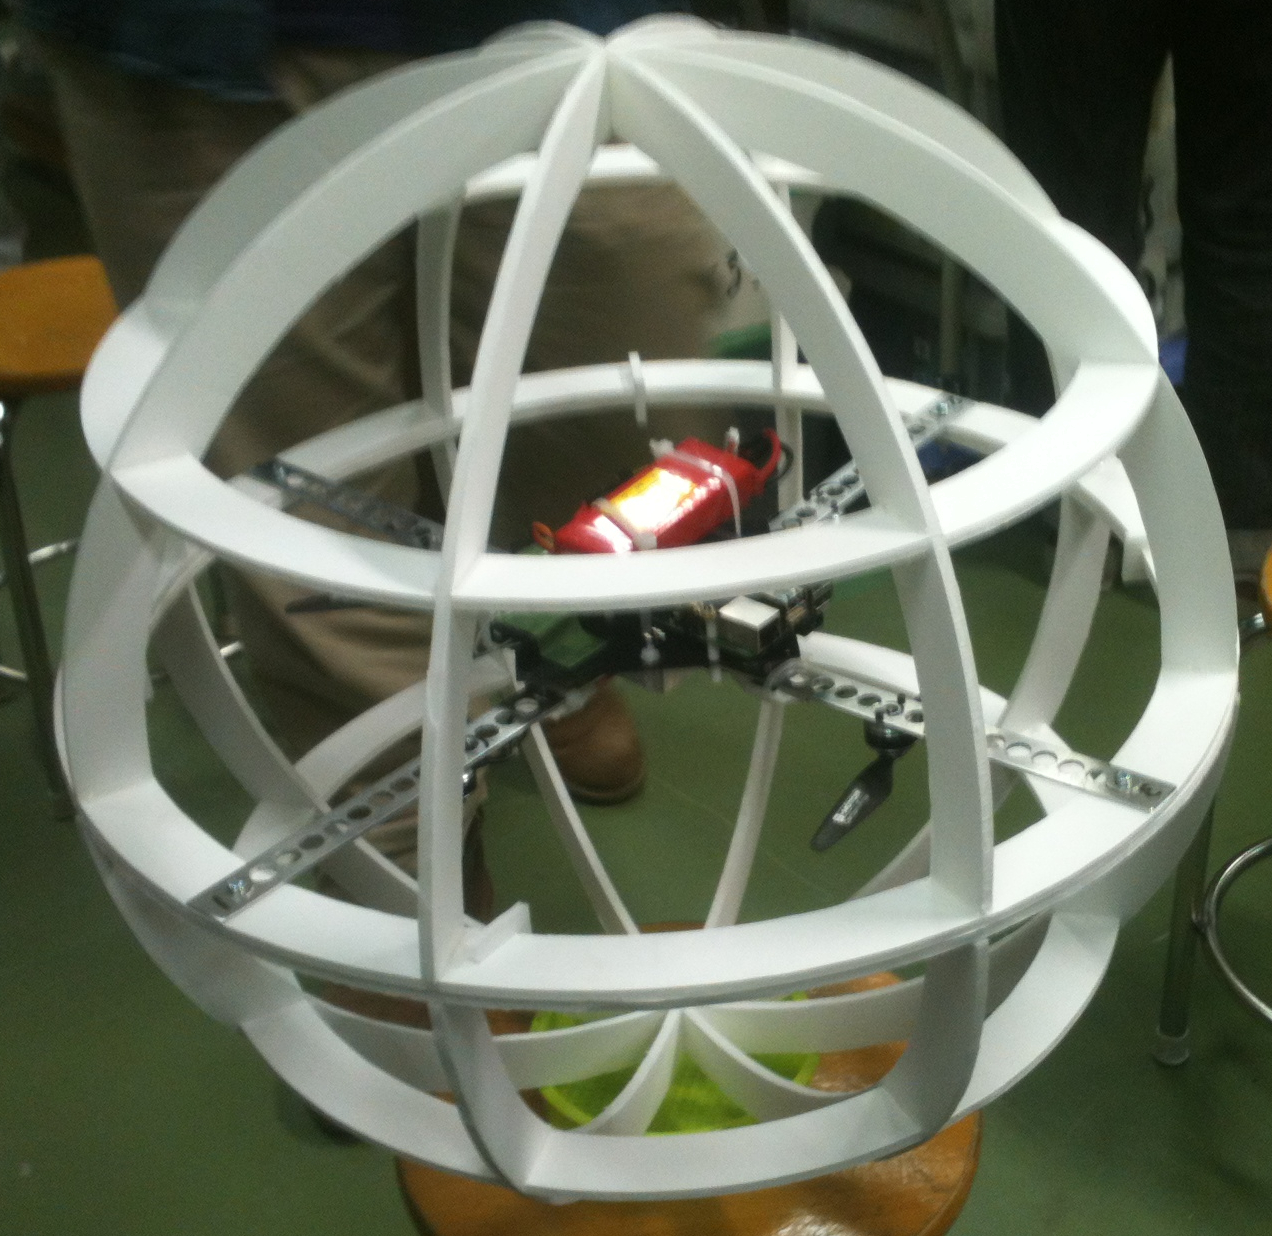
\includegraphics[width=50mm]{image/1.JPG}
  \caption{球体ドローン1号機}
  \label{fig:1}
 \end{center}
\end{figure*}

\begin{figure*}[b]
 \begin{center}
  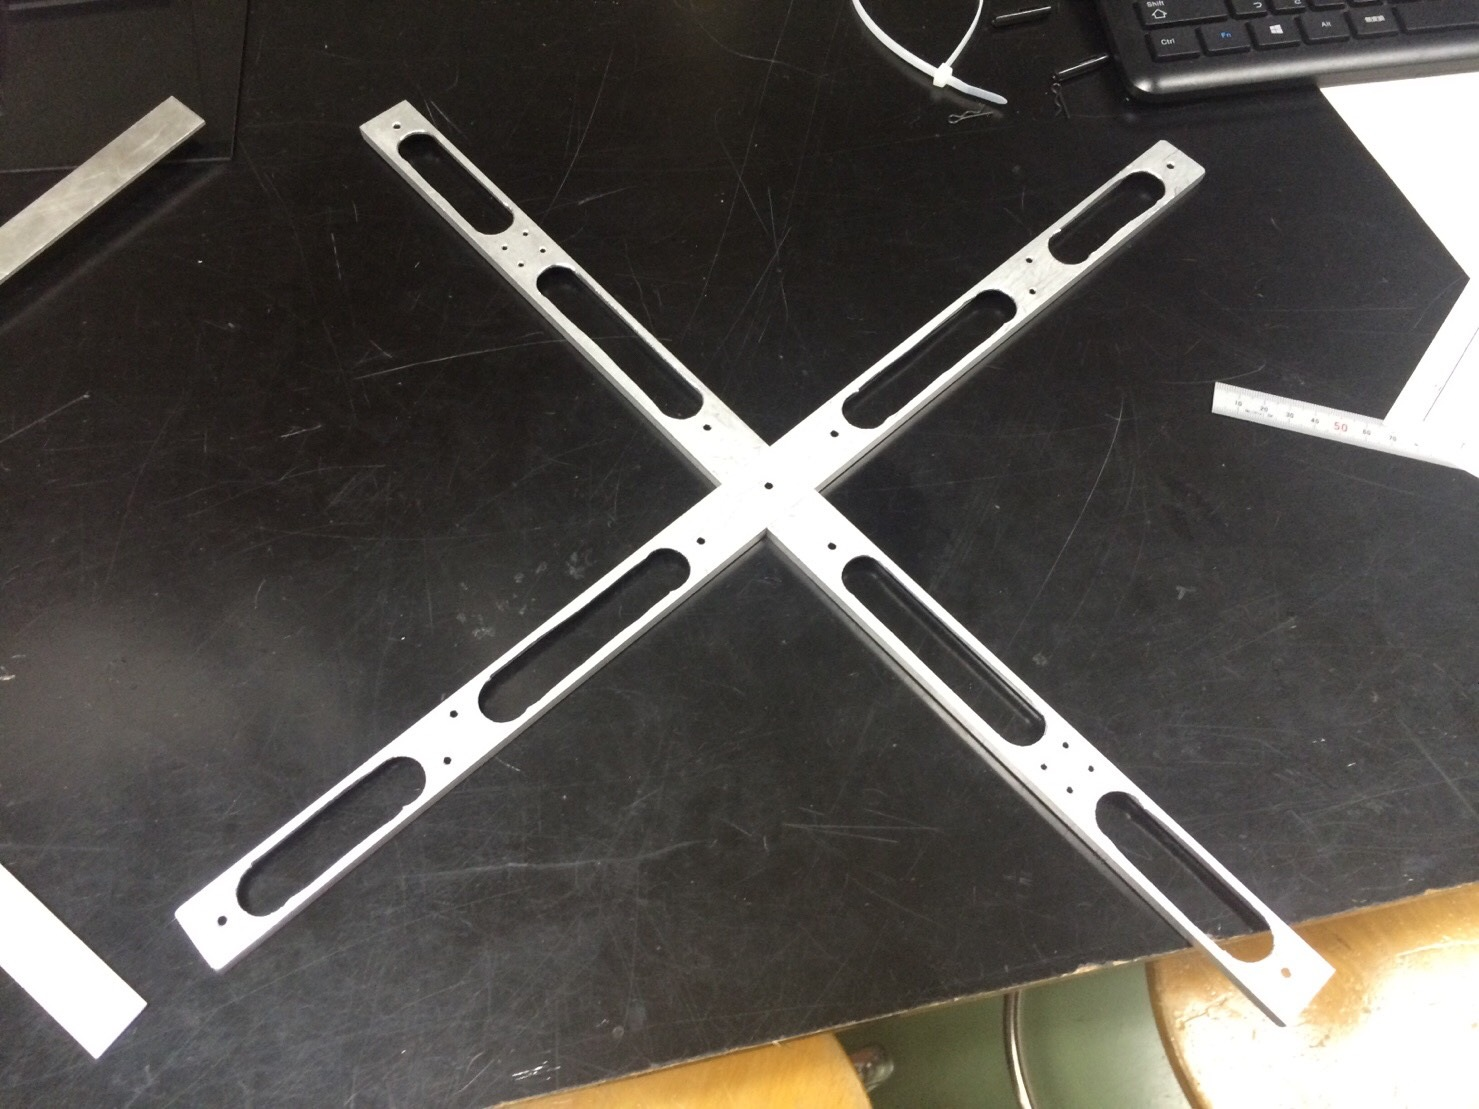
\includegraphics[width=50mm]{image/arm-2.JPG}
  \caption{改良したアーム}
  \label{fig:arm}
 \end{center}
\end{figure*}

\begin{figure*}[b]
 \begin{center}
  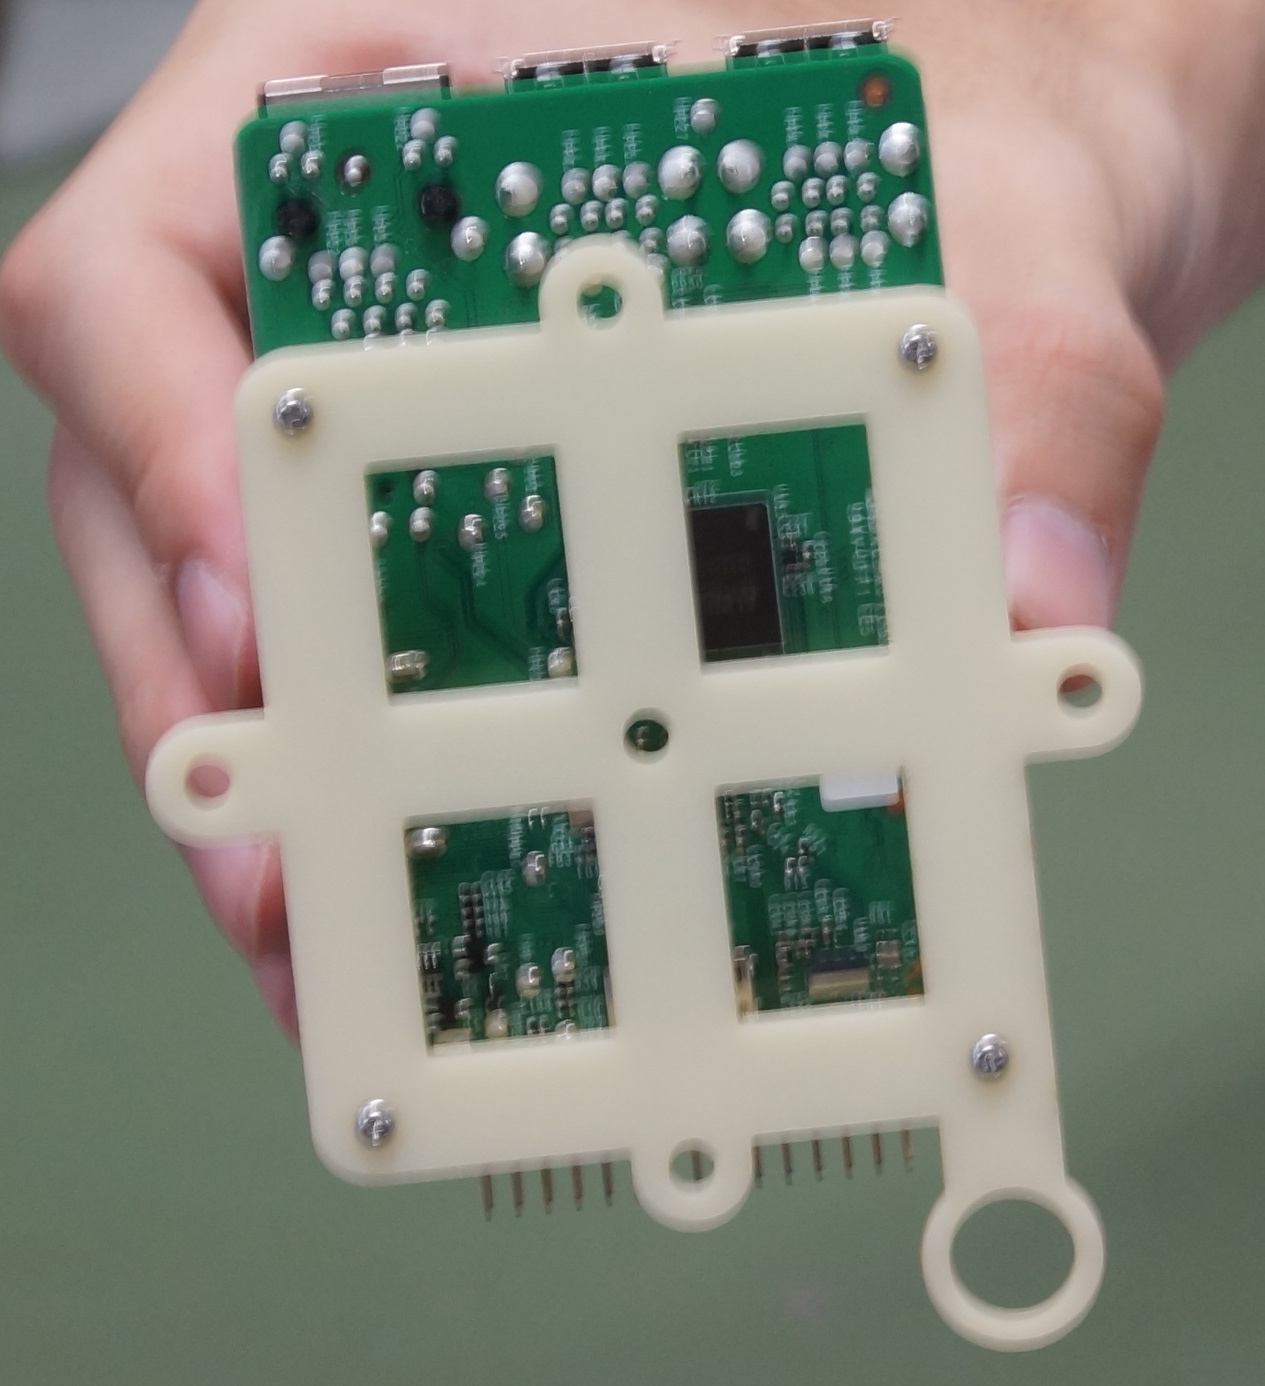
\includegraphics[width=50mm]{image/RPi-board-1.JPG}
  \caption{RPi取付板}
  \label{fig:RPi-board}
 \end{center}
\end{figure*}

\begin{figure*}[b]
 \begin{center}
  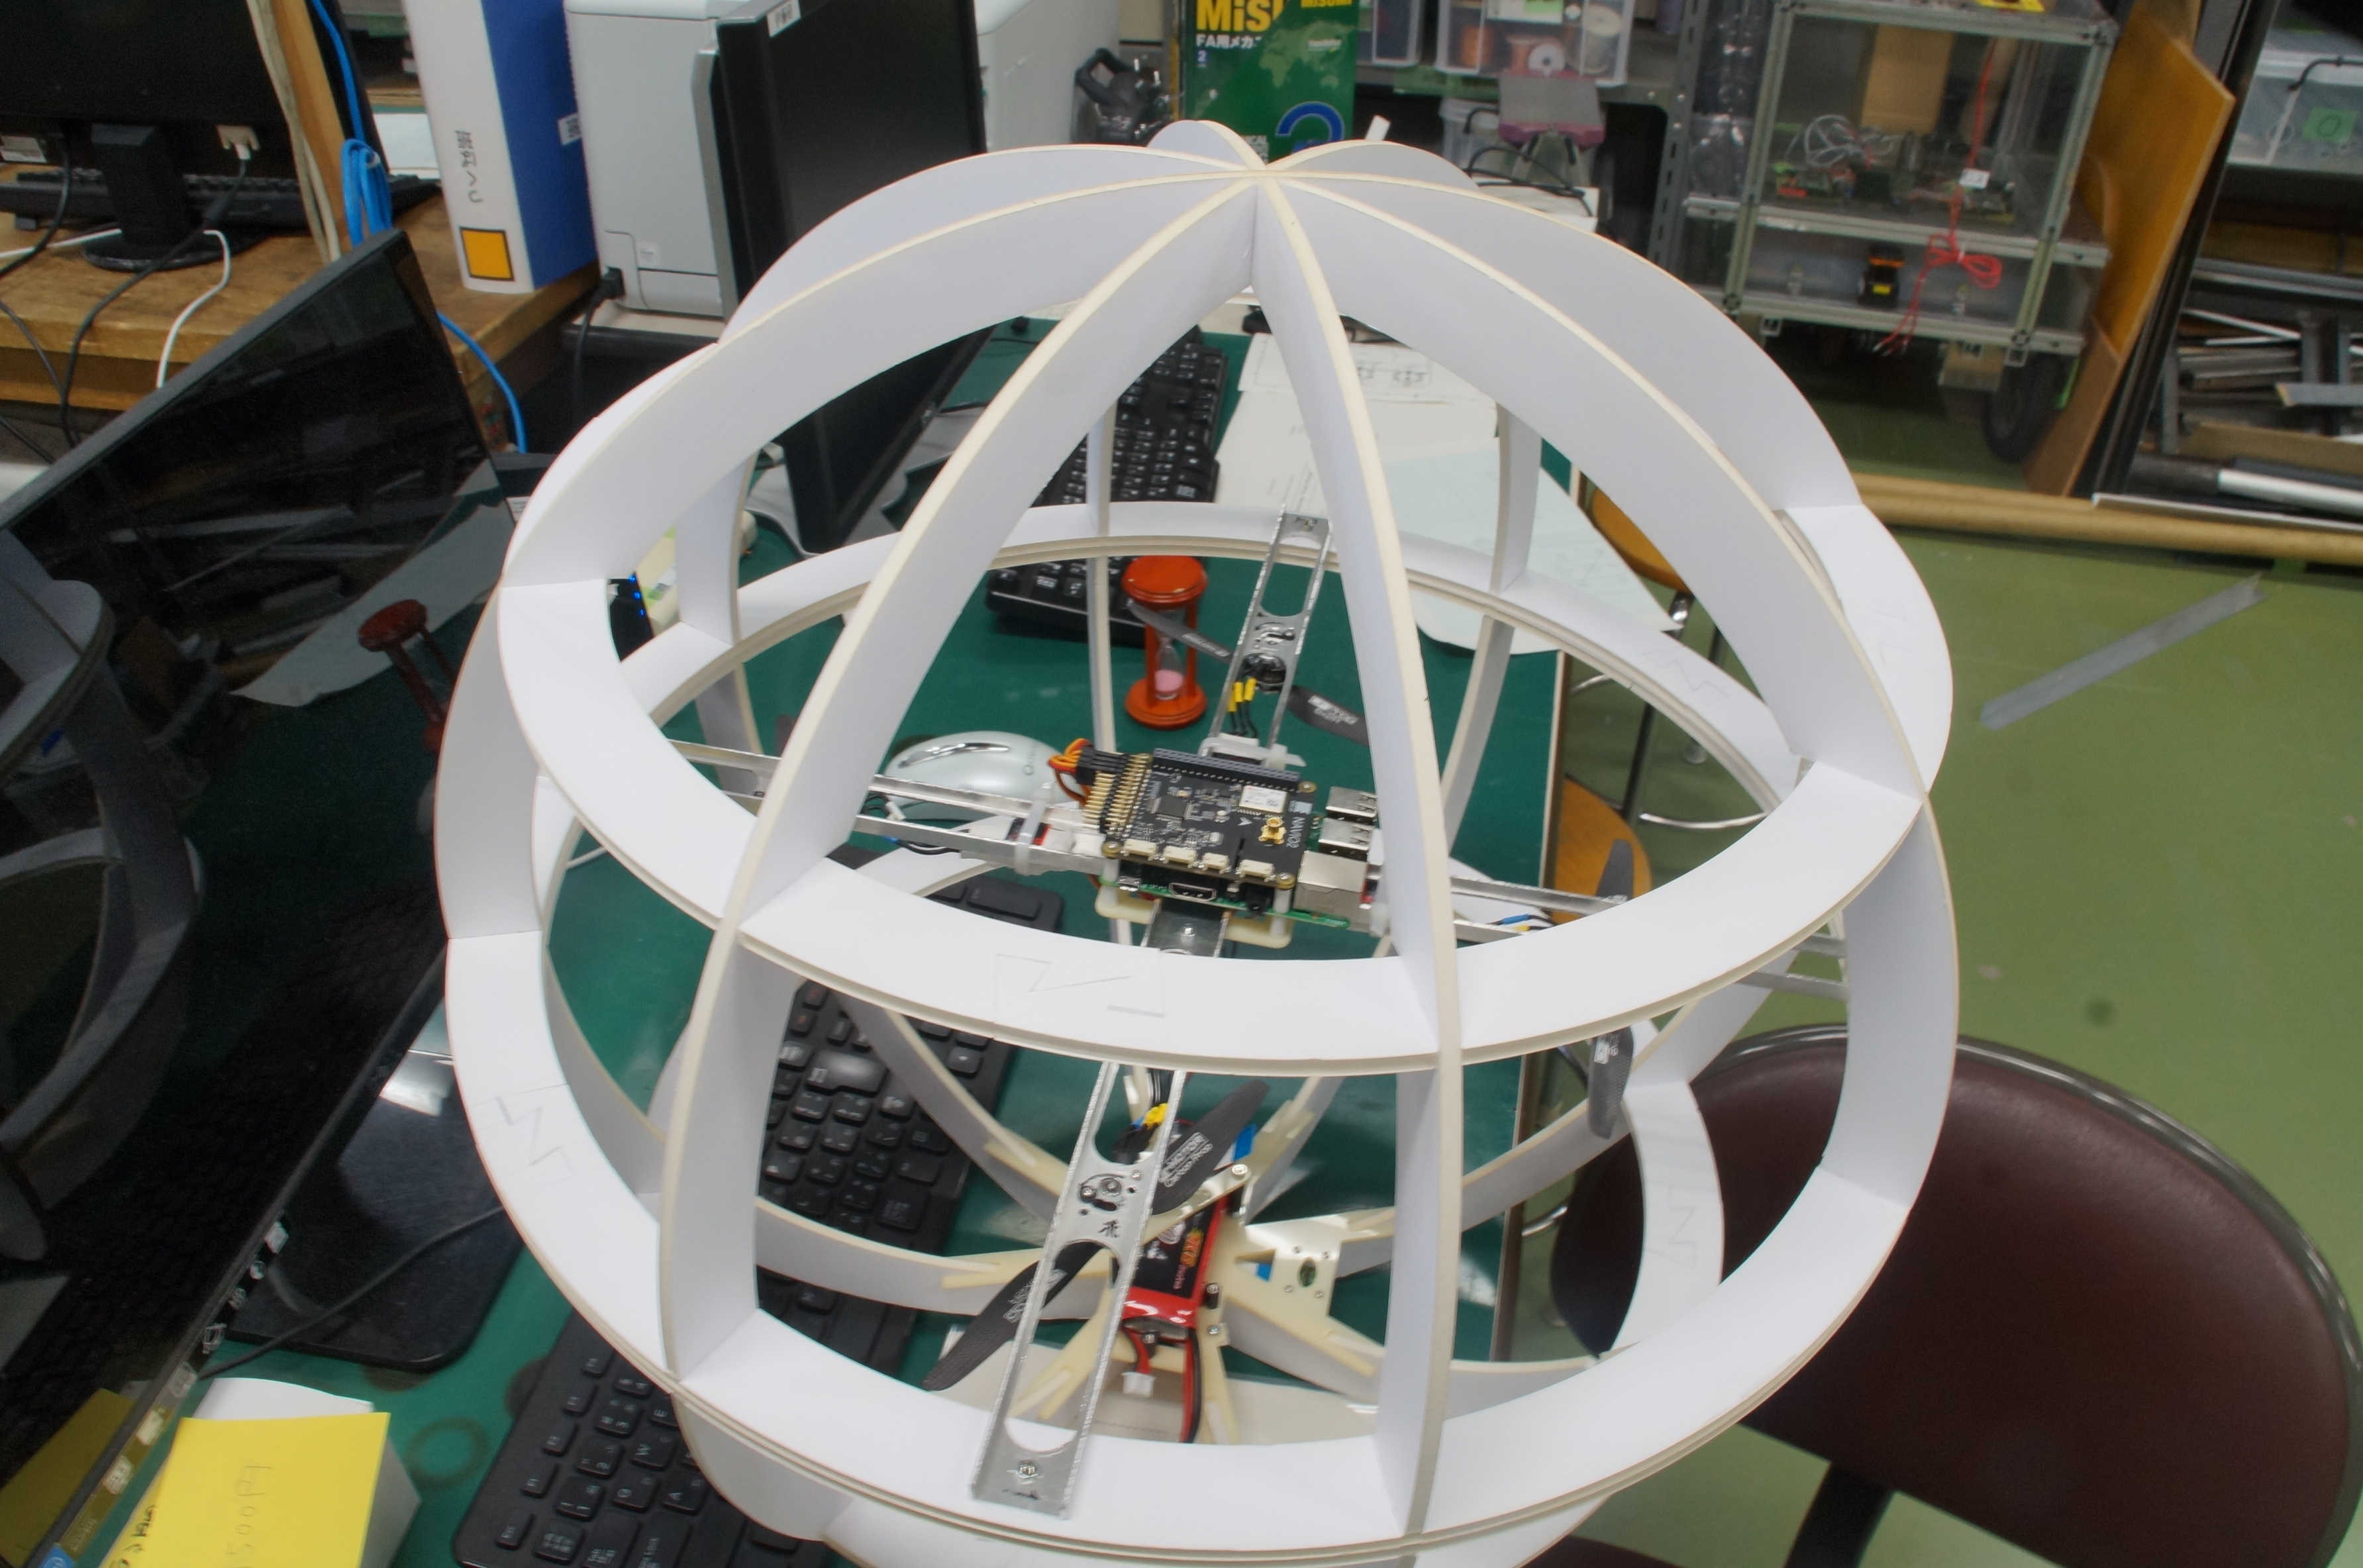
\includegraphics[width=50mm]{image/3.JPG}
  \caption{球体ドローン3号機}
  \label{fig:3}
 \end{center}
\end{figure*}

\begin{figure*}[b]
 \begin{center}
  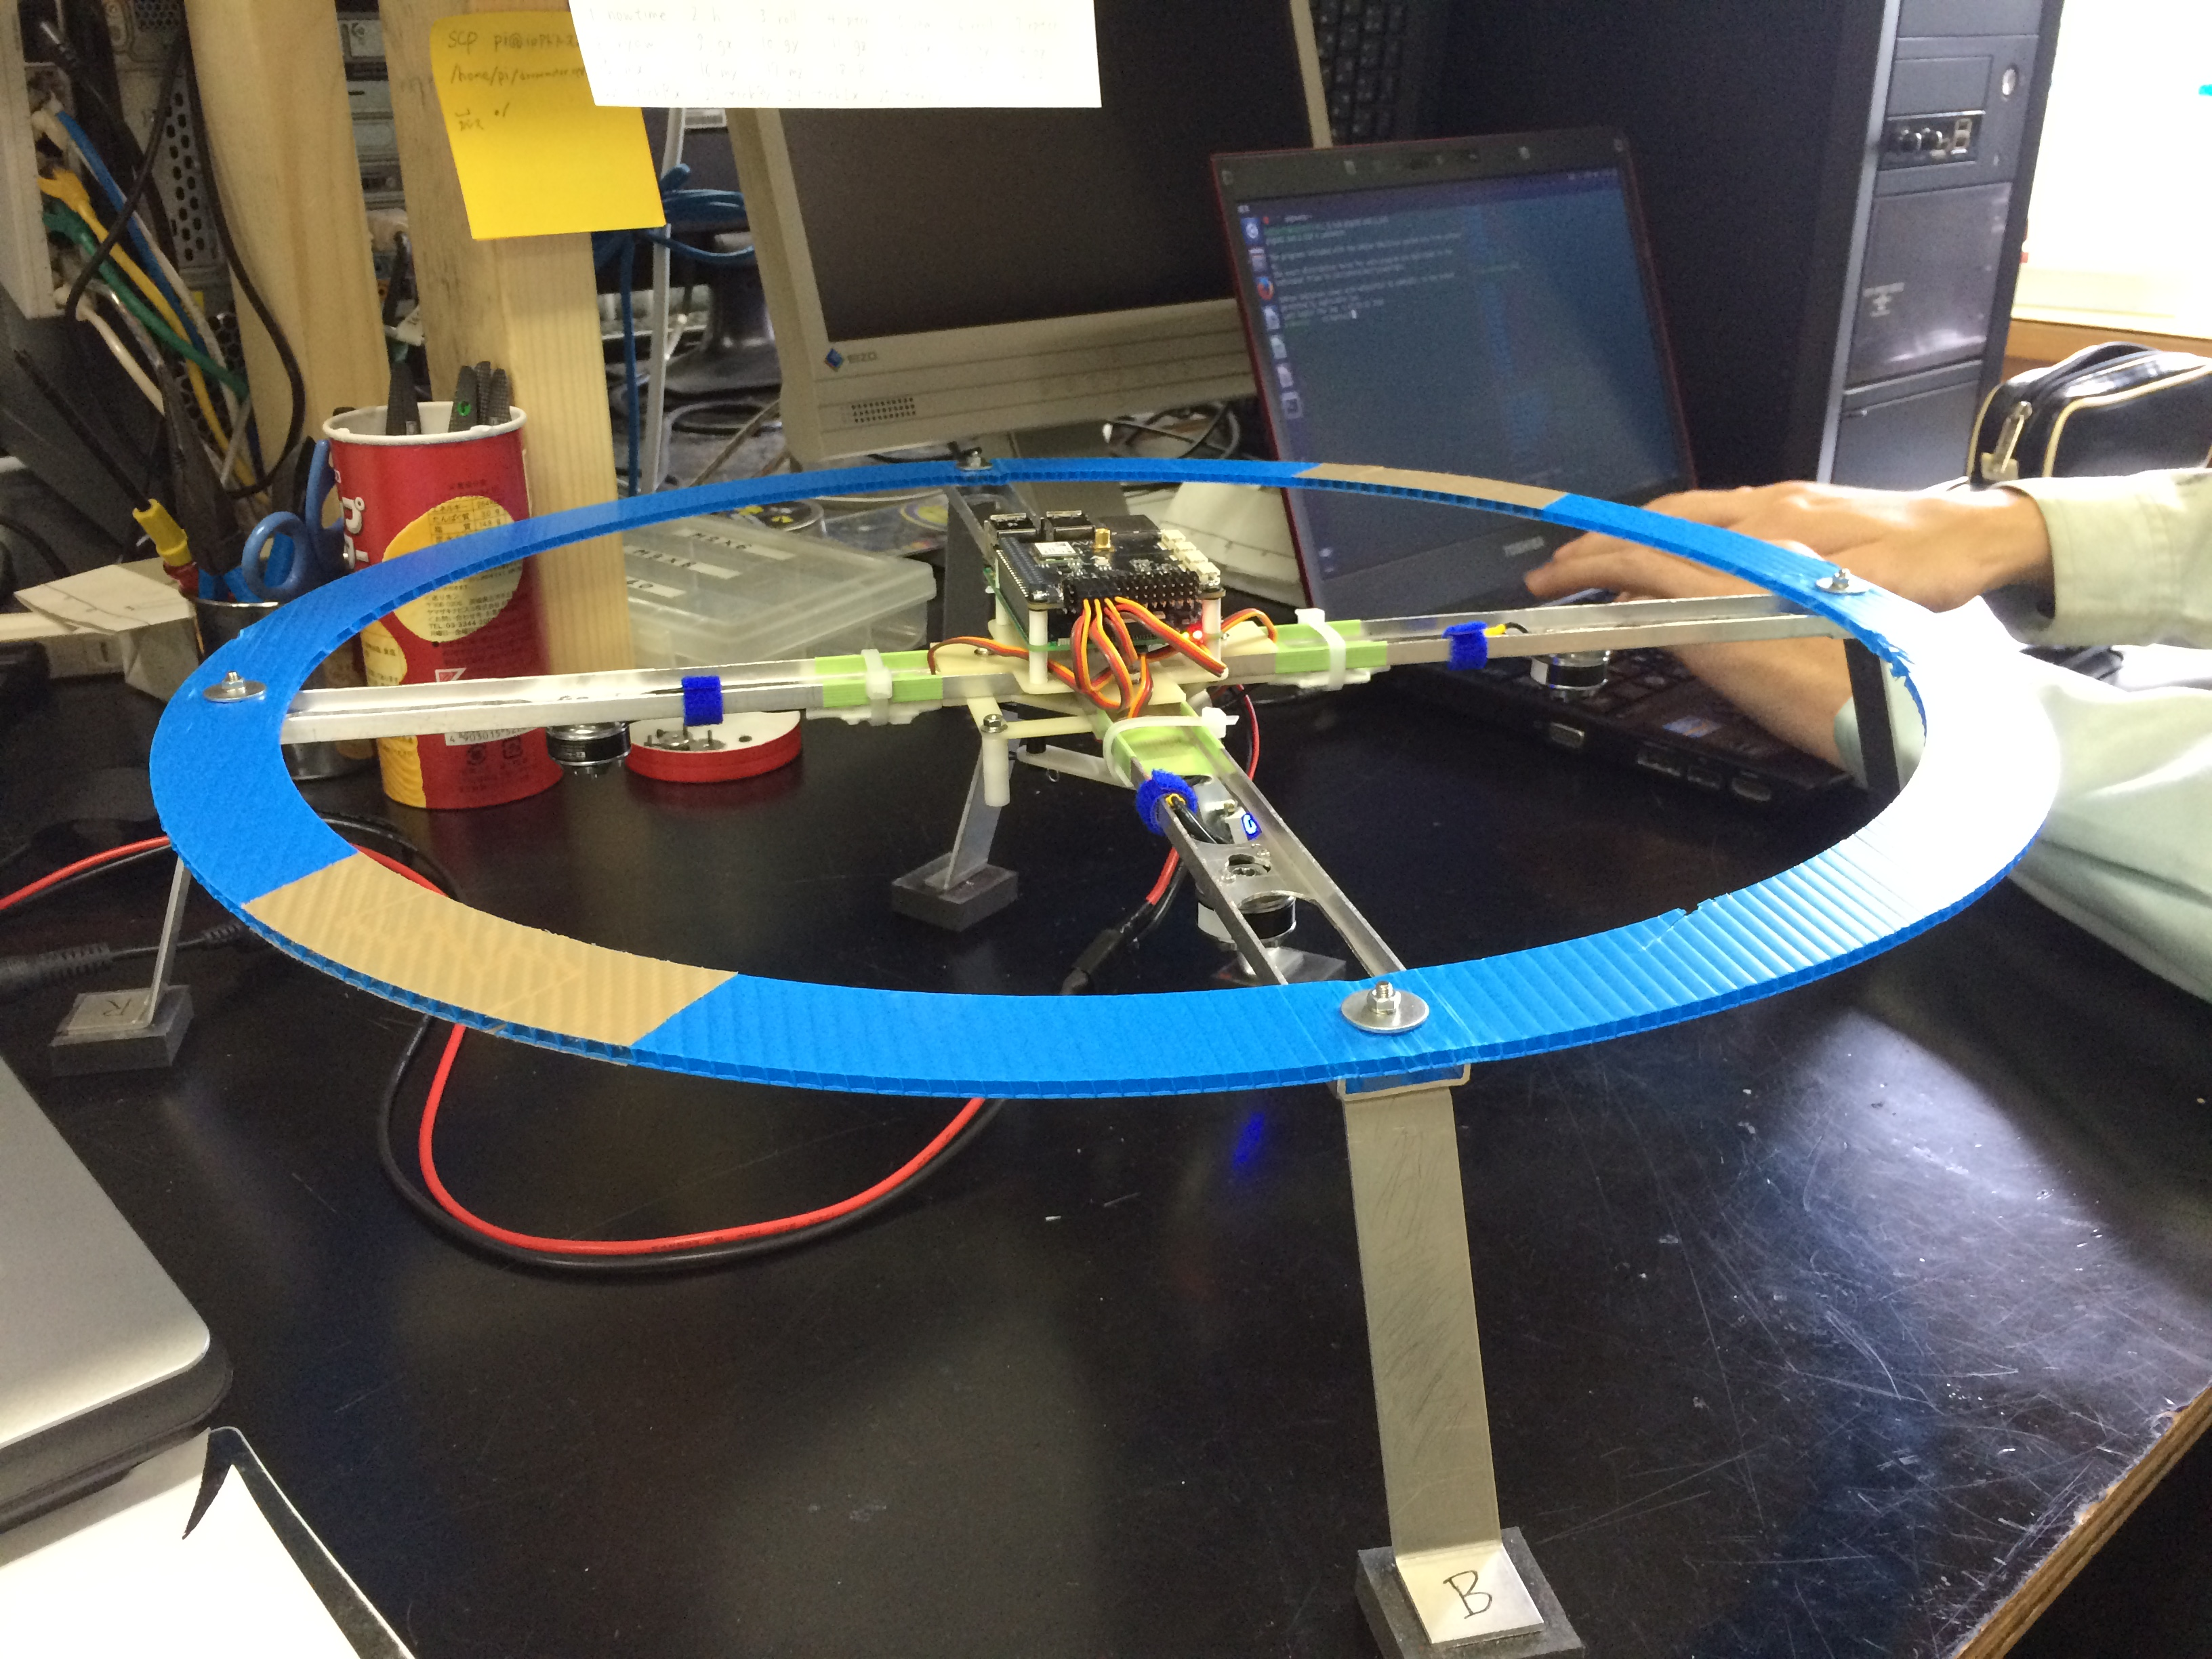
\includegraphics[width=50mm]{image/test-machine.JPG}
  \caption{制御実験機}
  \label{fig:test-machine}
 \end{center}
\end{figure*}

\begin{figure*}[b]
 \begin{center}
  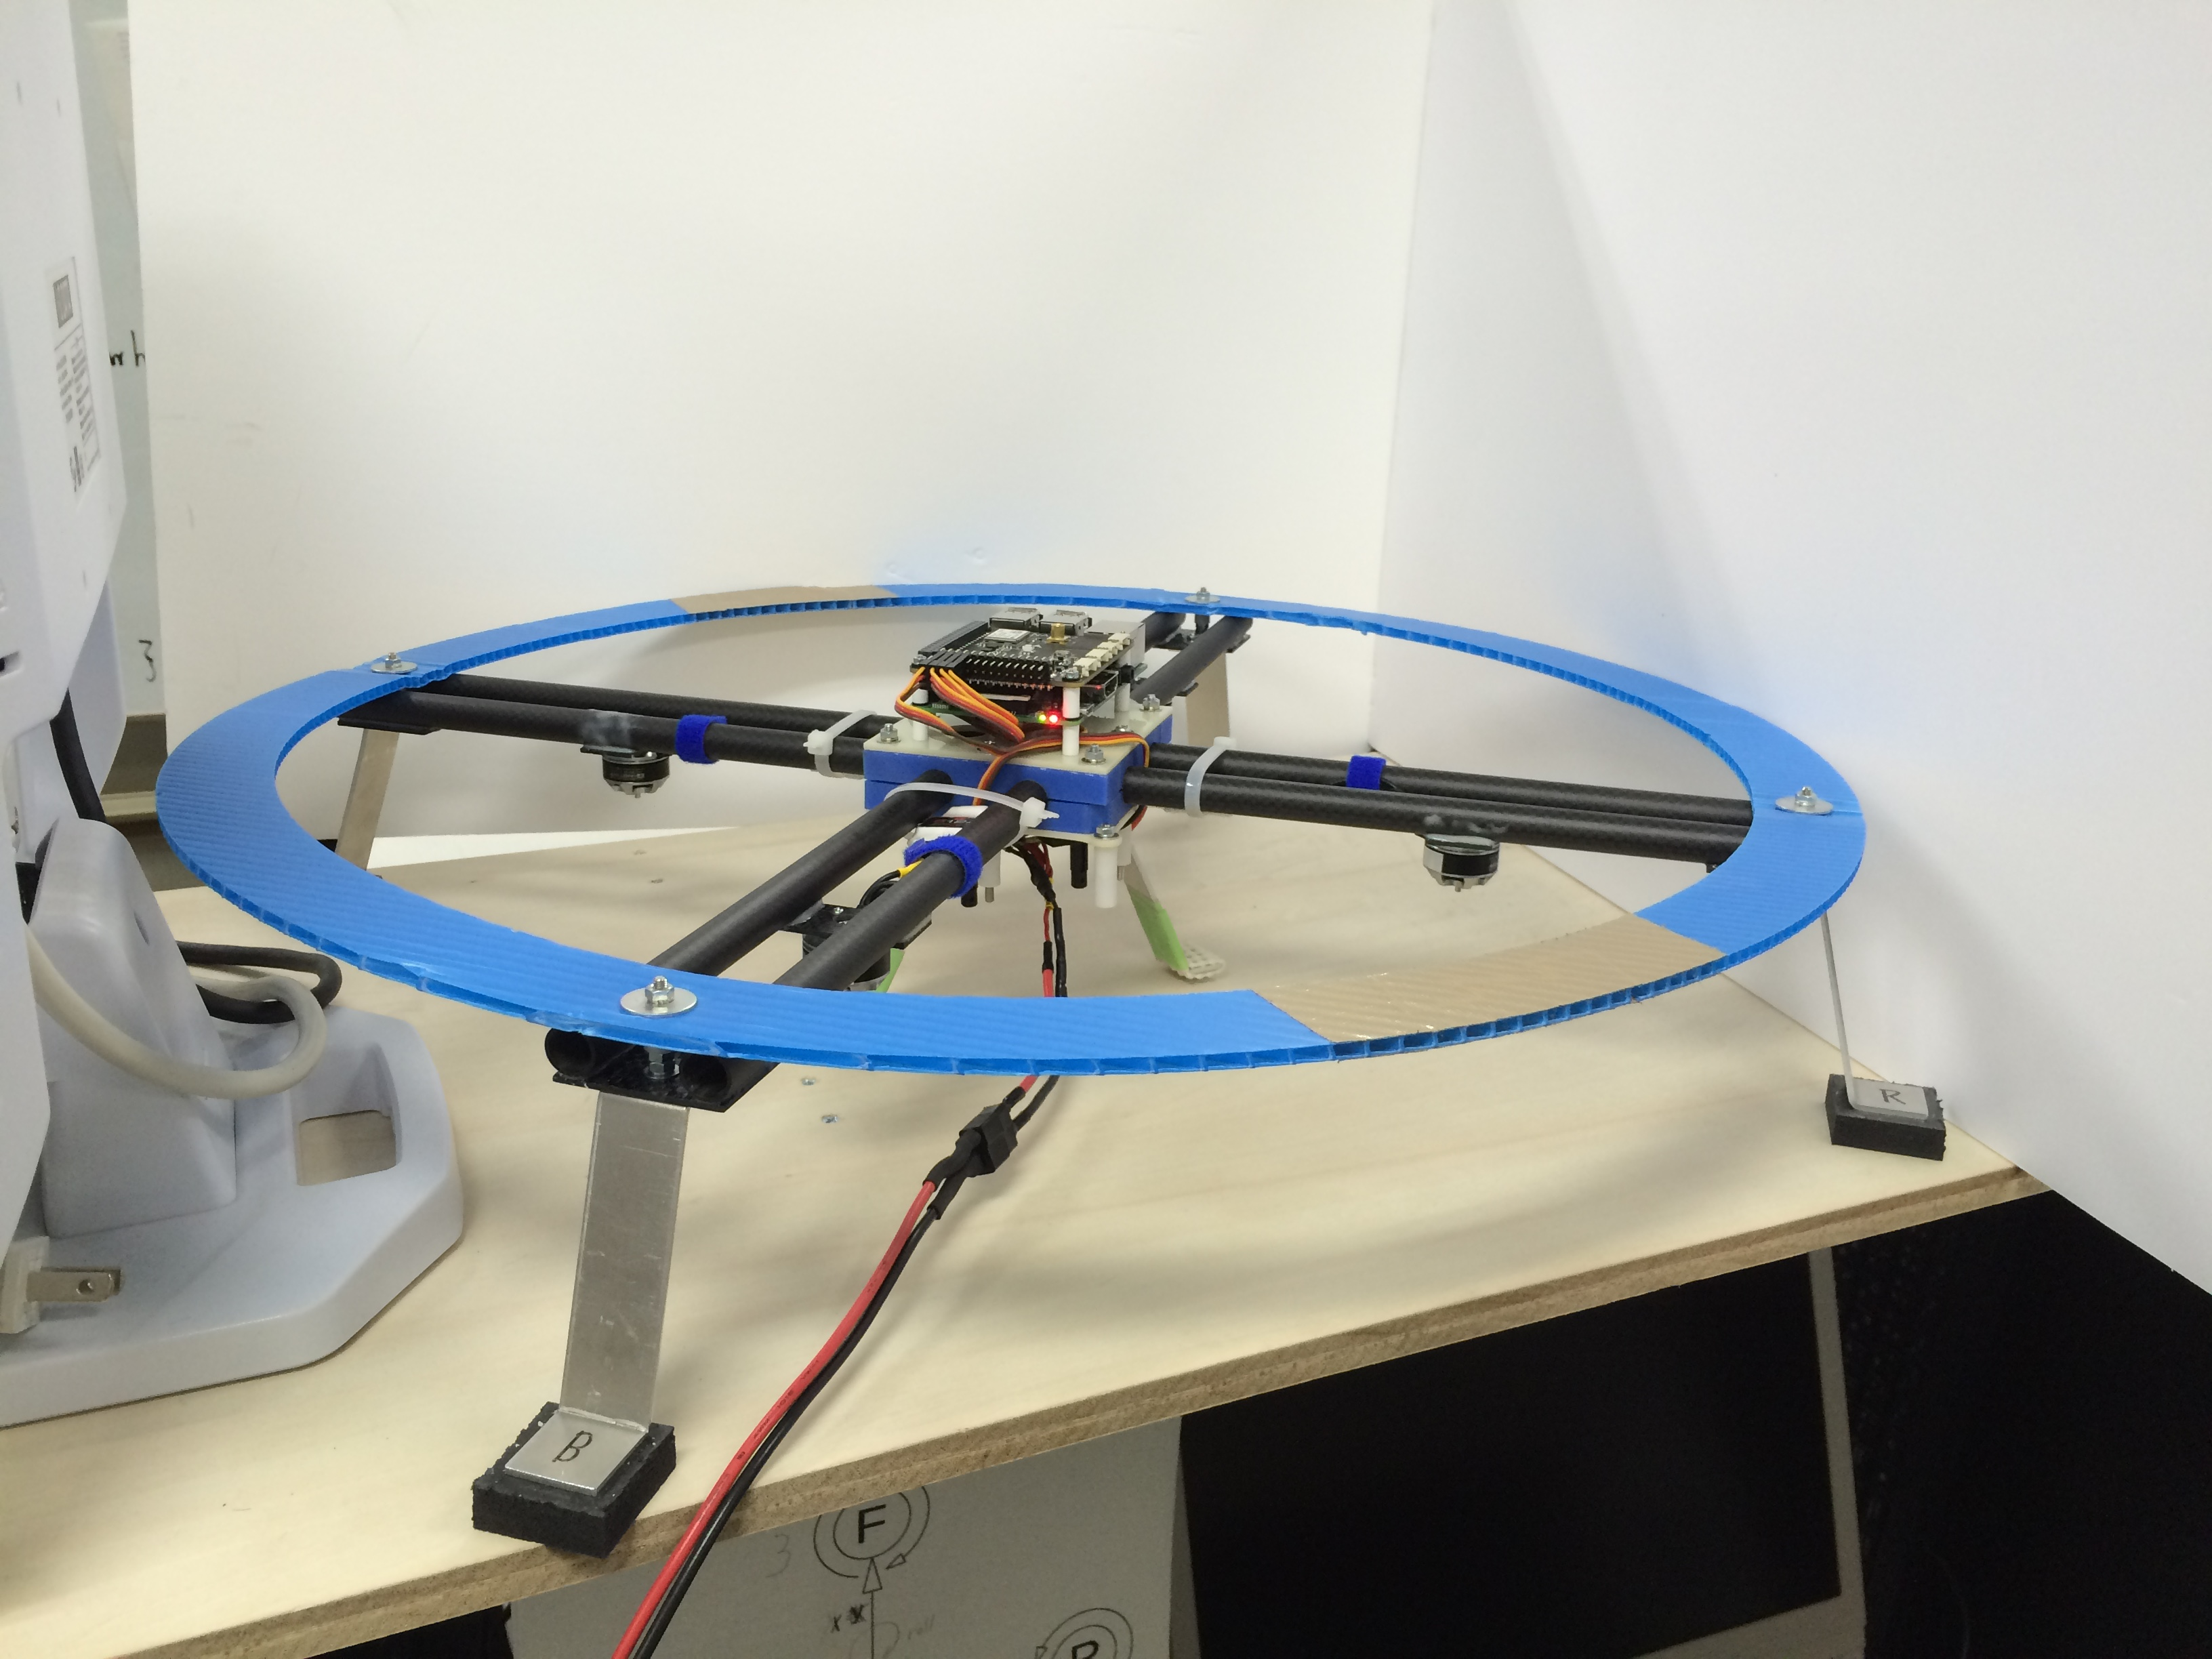
\includegraphics[width=50mm]{image/drone-4.JPG}
  \caption{本機体1号機}
  \label{fig:drone-4}
 \end{center}
\end{figure*}

\begin{figure*}[b]
 \begin{center}
  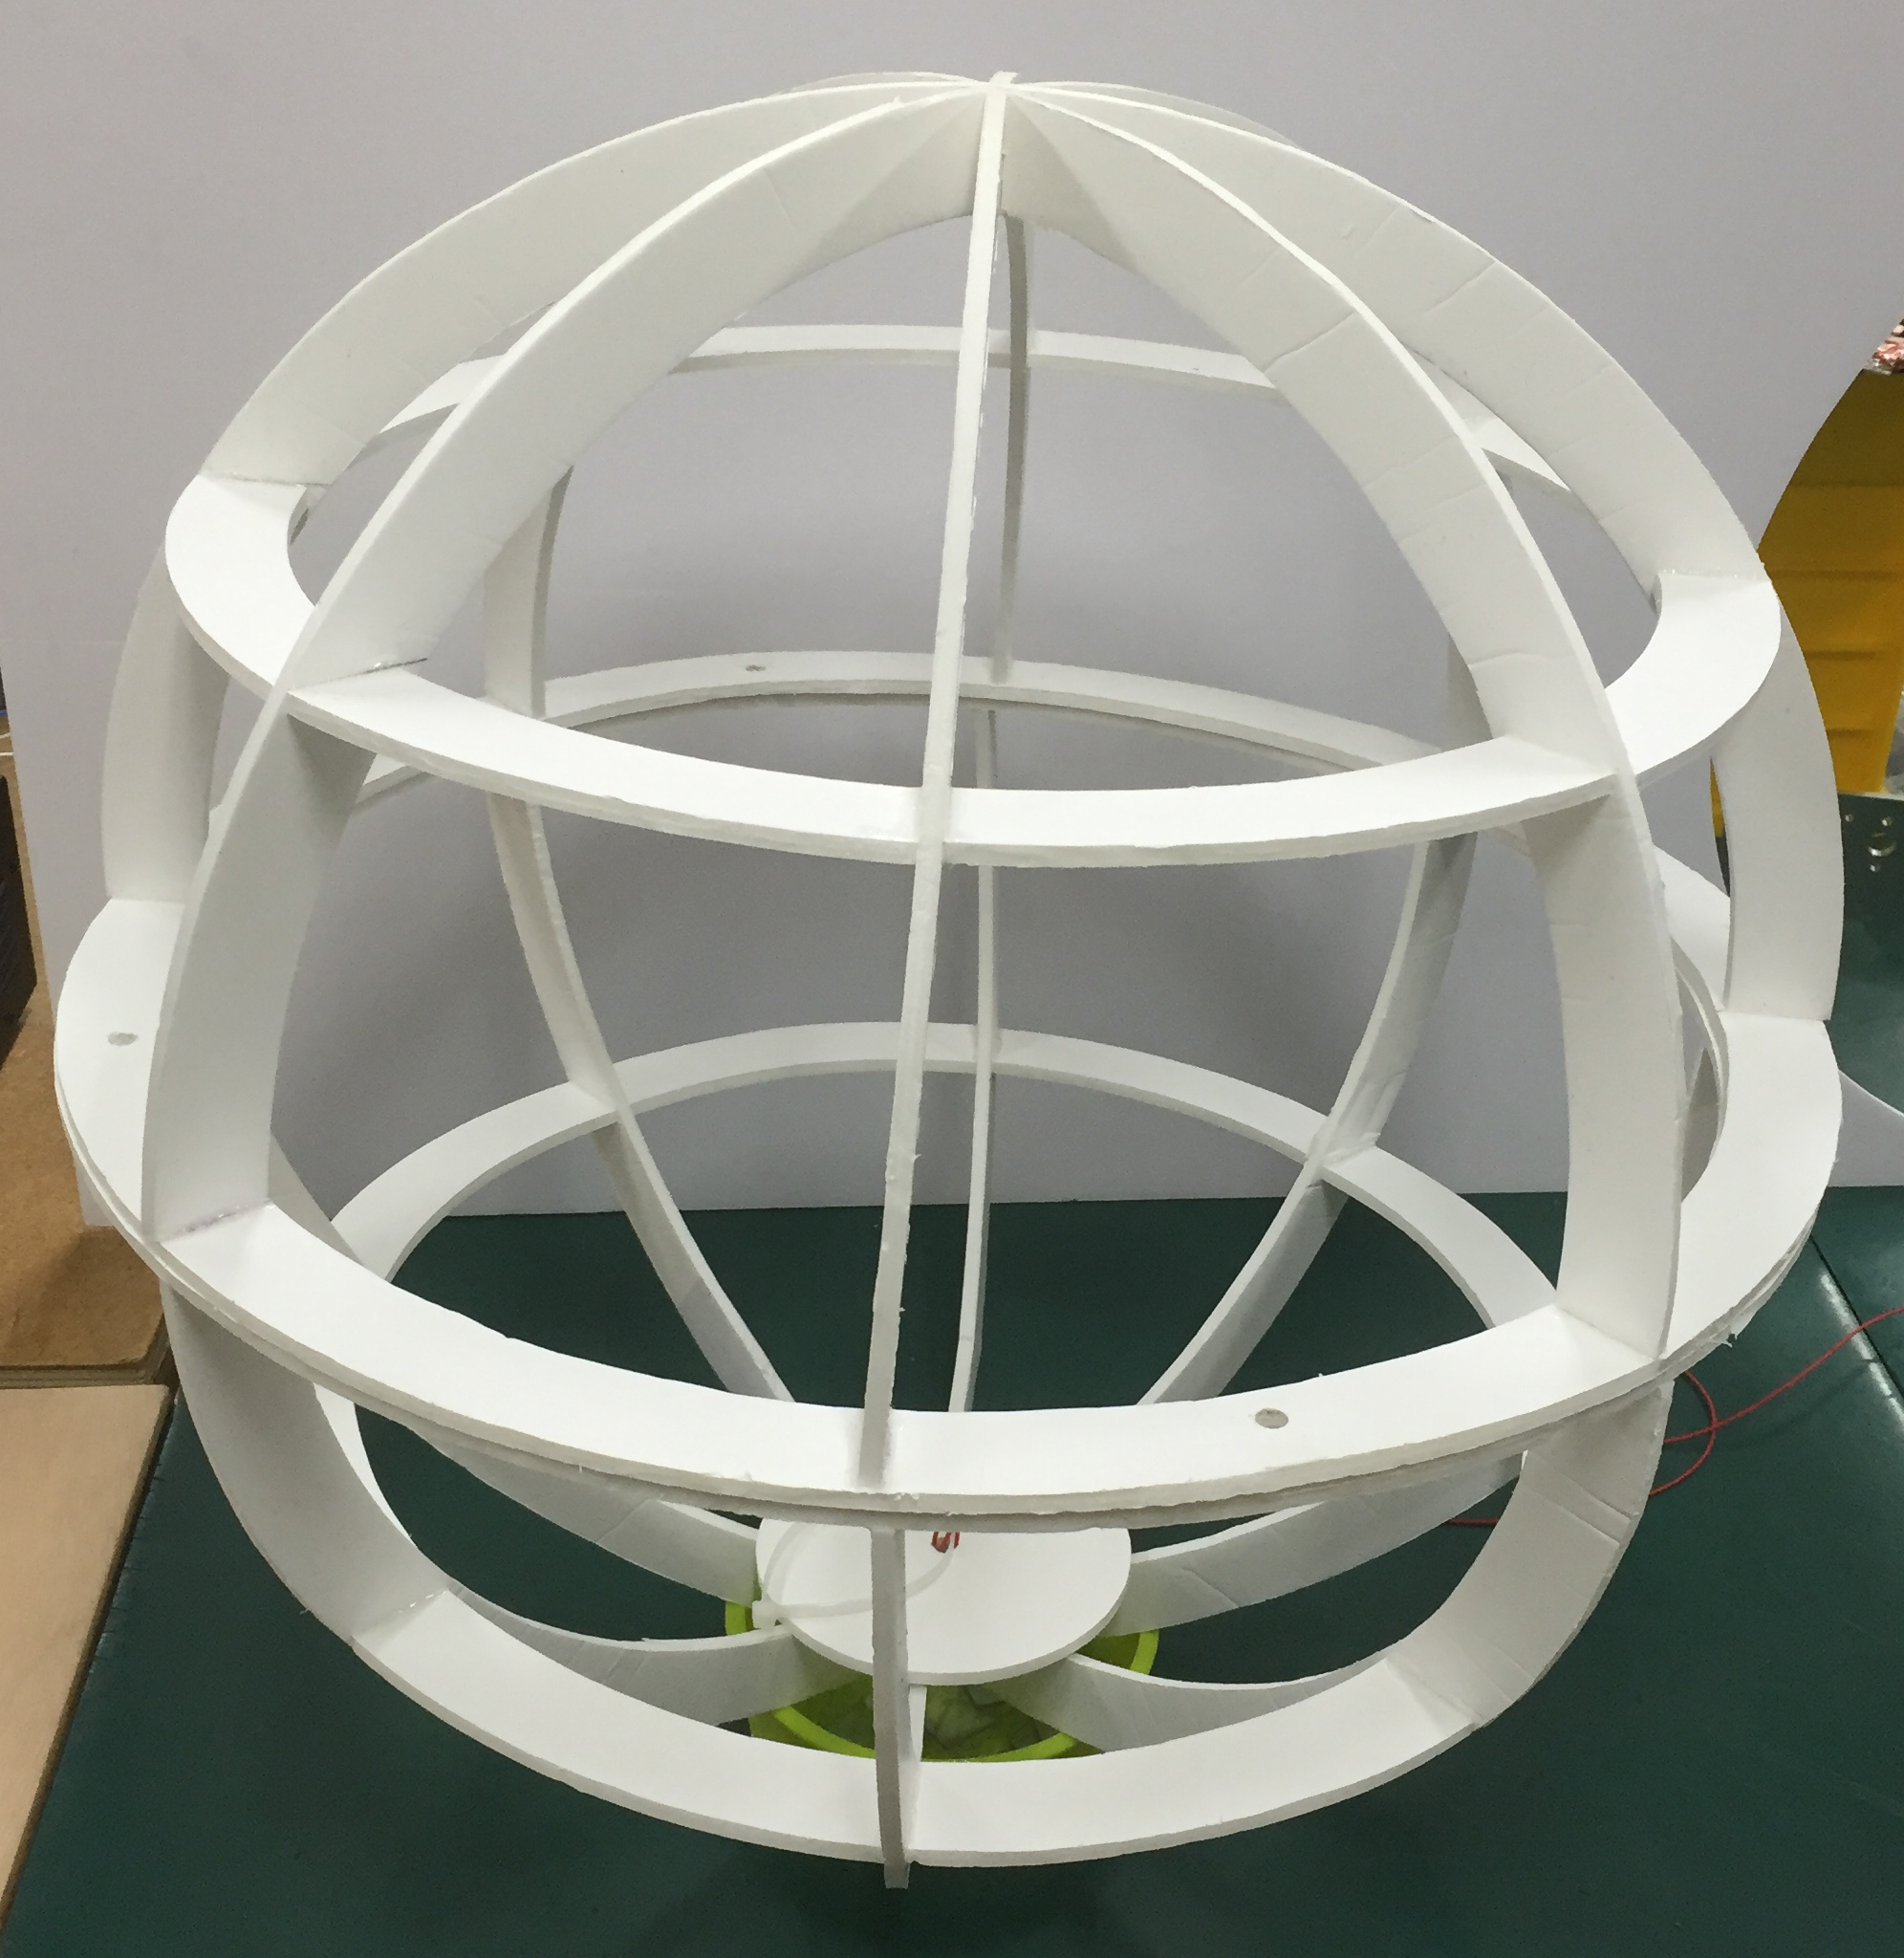
\includegraphics[width=50mm]{image/sphere-1.JPG}
  \caption{球体1号機}
  \label{fig:sphere-1}
 \end{center}
\end{figure*}

\begin{figure*}[b]
 \begin{center}
  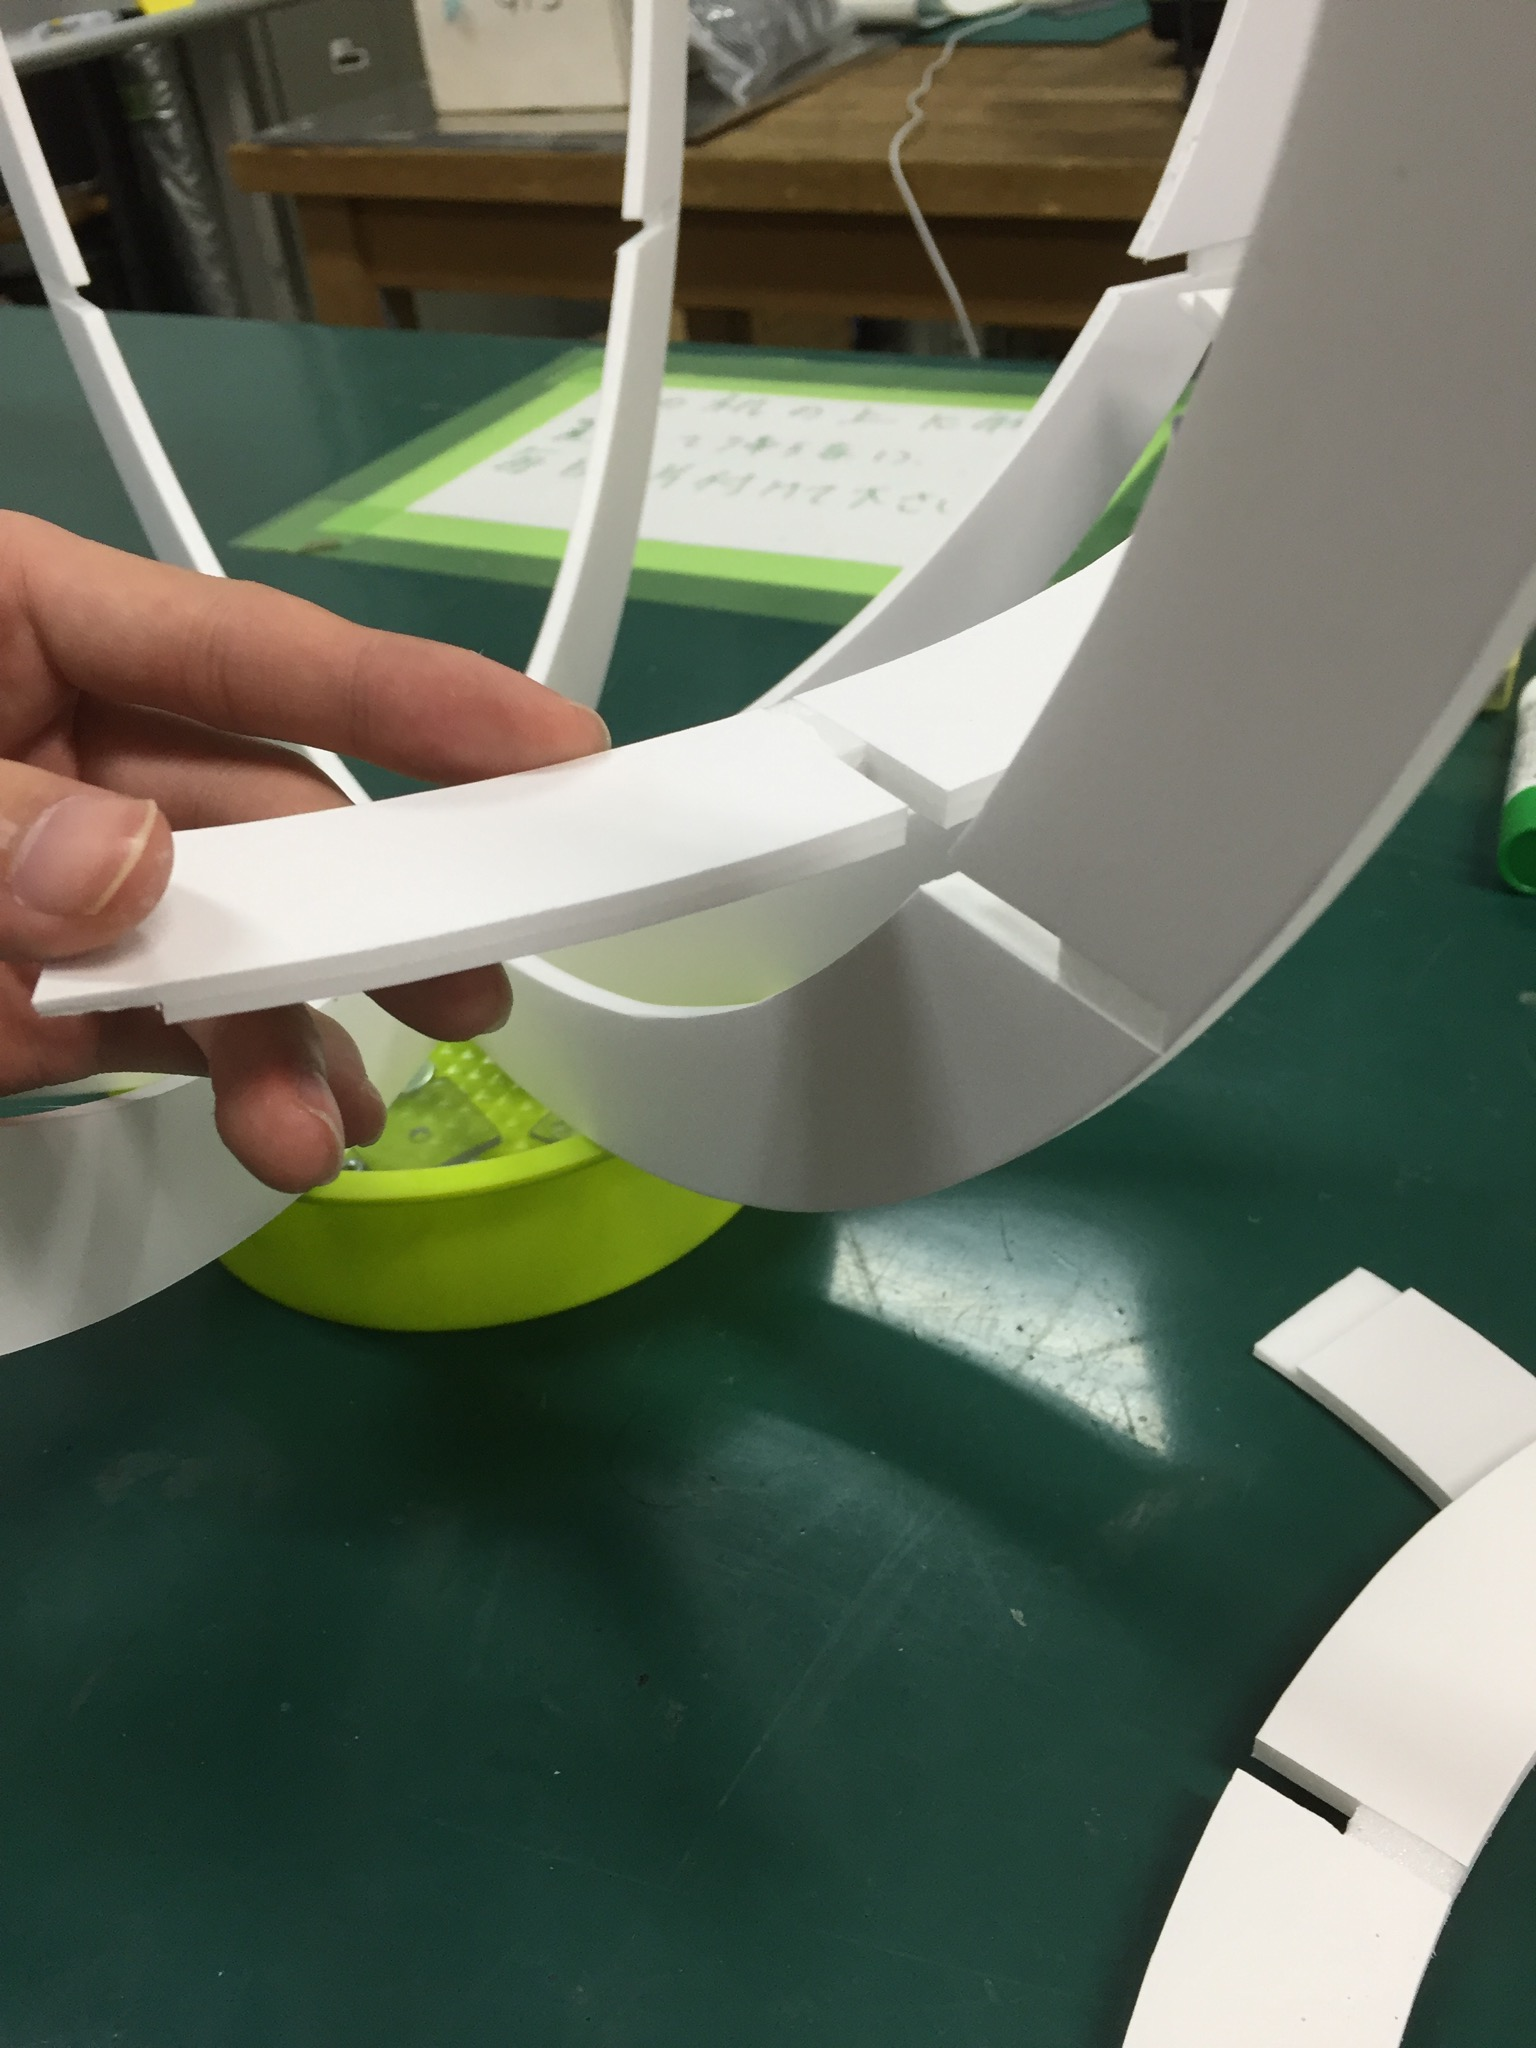
\includegraphics[width=50mm]{image/kigumi.JPG}
  \caption{木組み部分}
  \label{fig:kigumi}
 \end{center}
\end{figure*}

\begin{figure*}[b]
 \begin{center}
  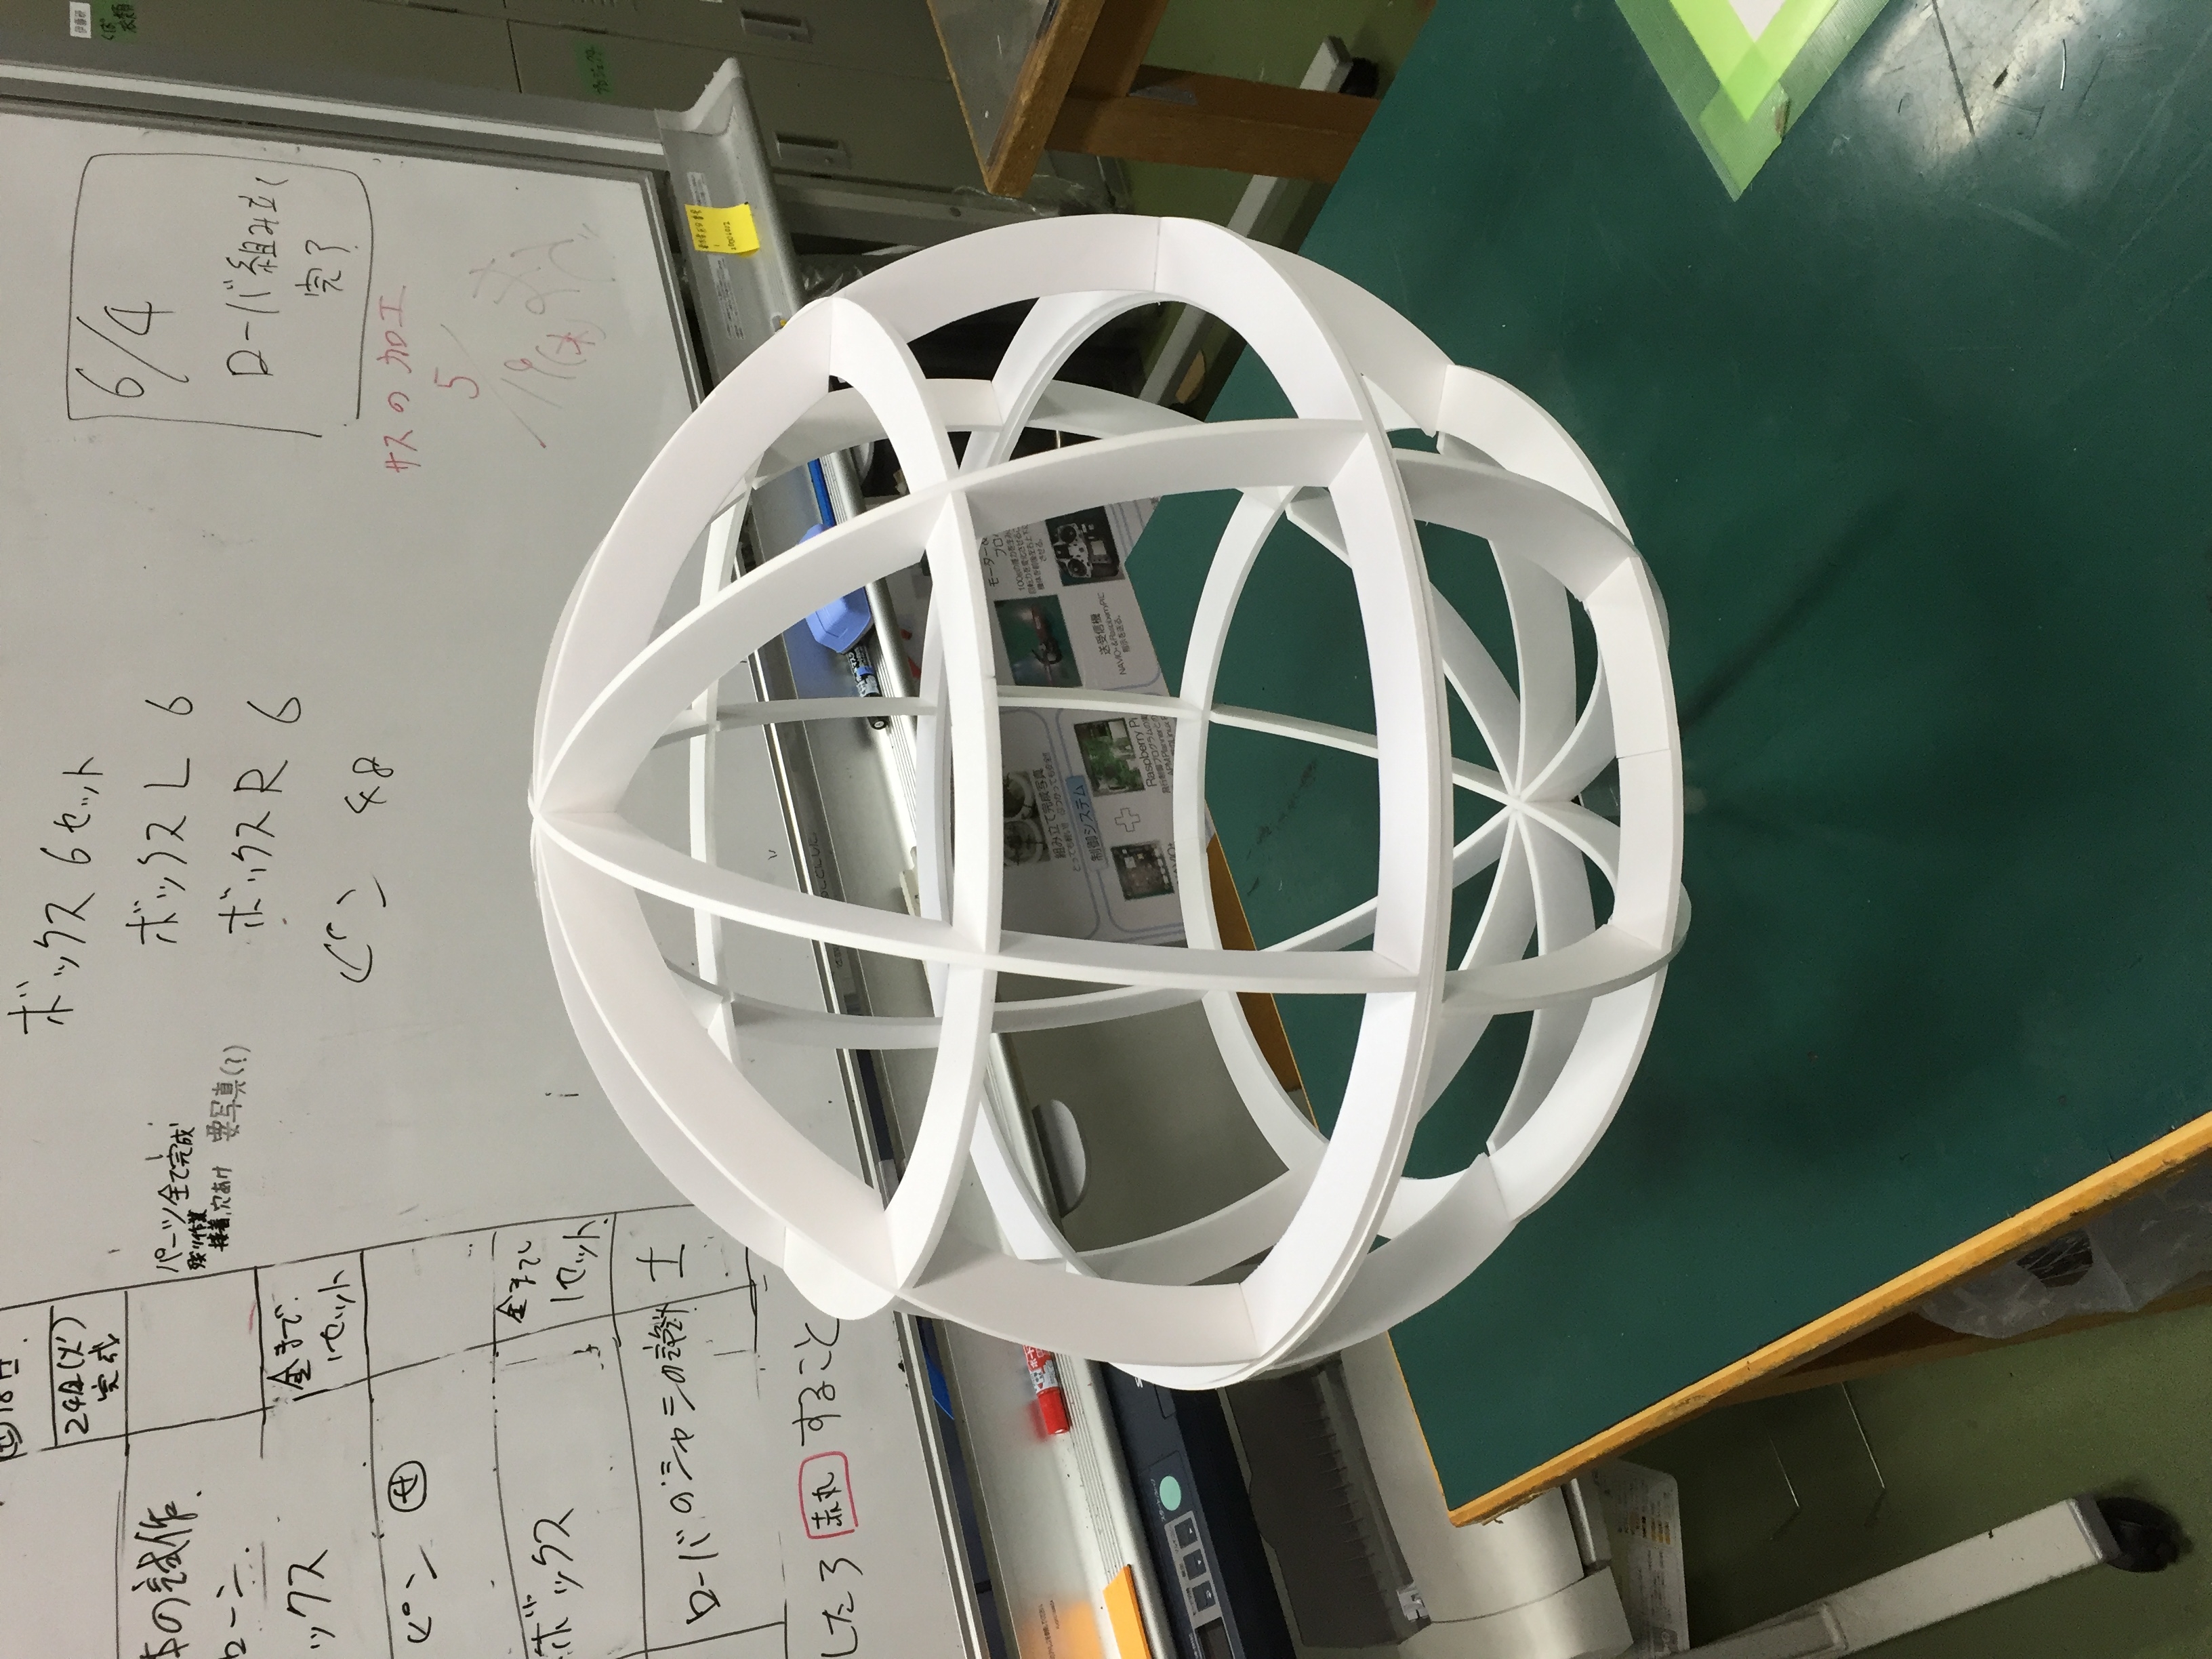
\includegraphics[width=50mm]{image/sphere-2.JPG}
  \caption{球体2号機}
  \label{fig:sphere-2}
 \end{center}
\end{figure*}

\begin{figure*}[b]
 \begin{center}
  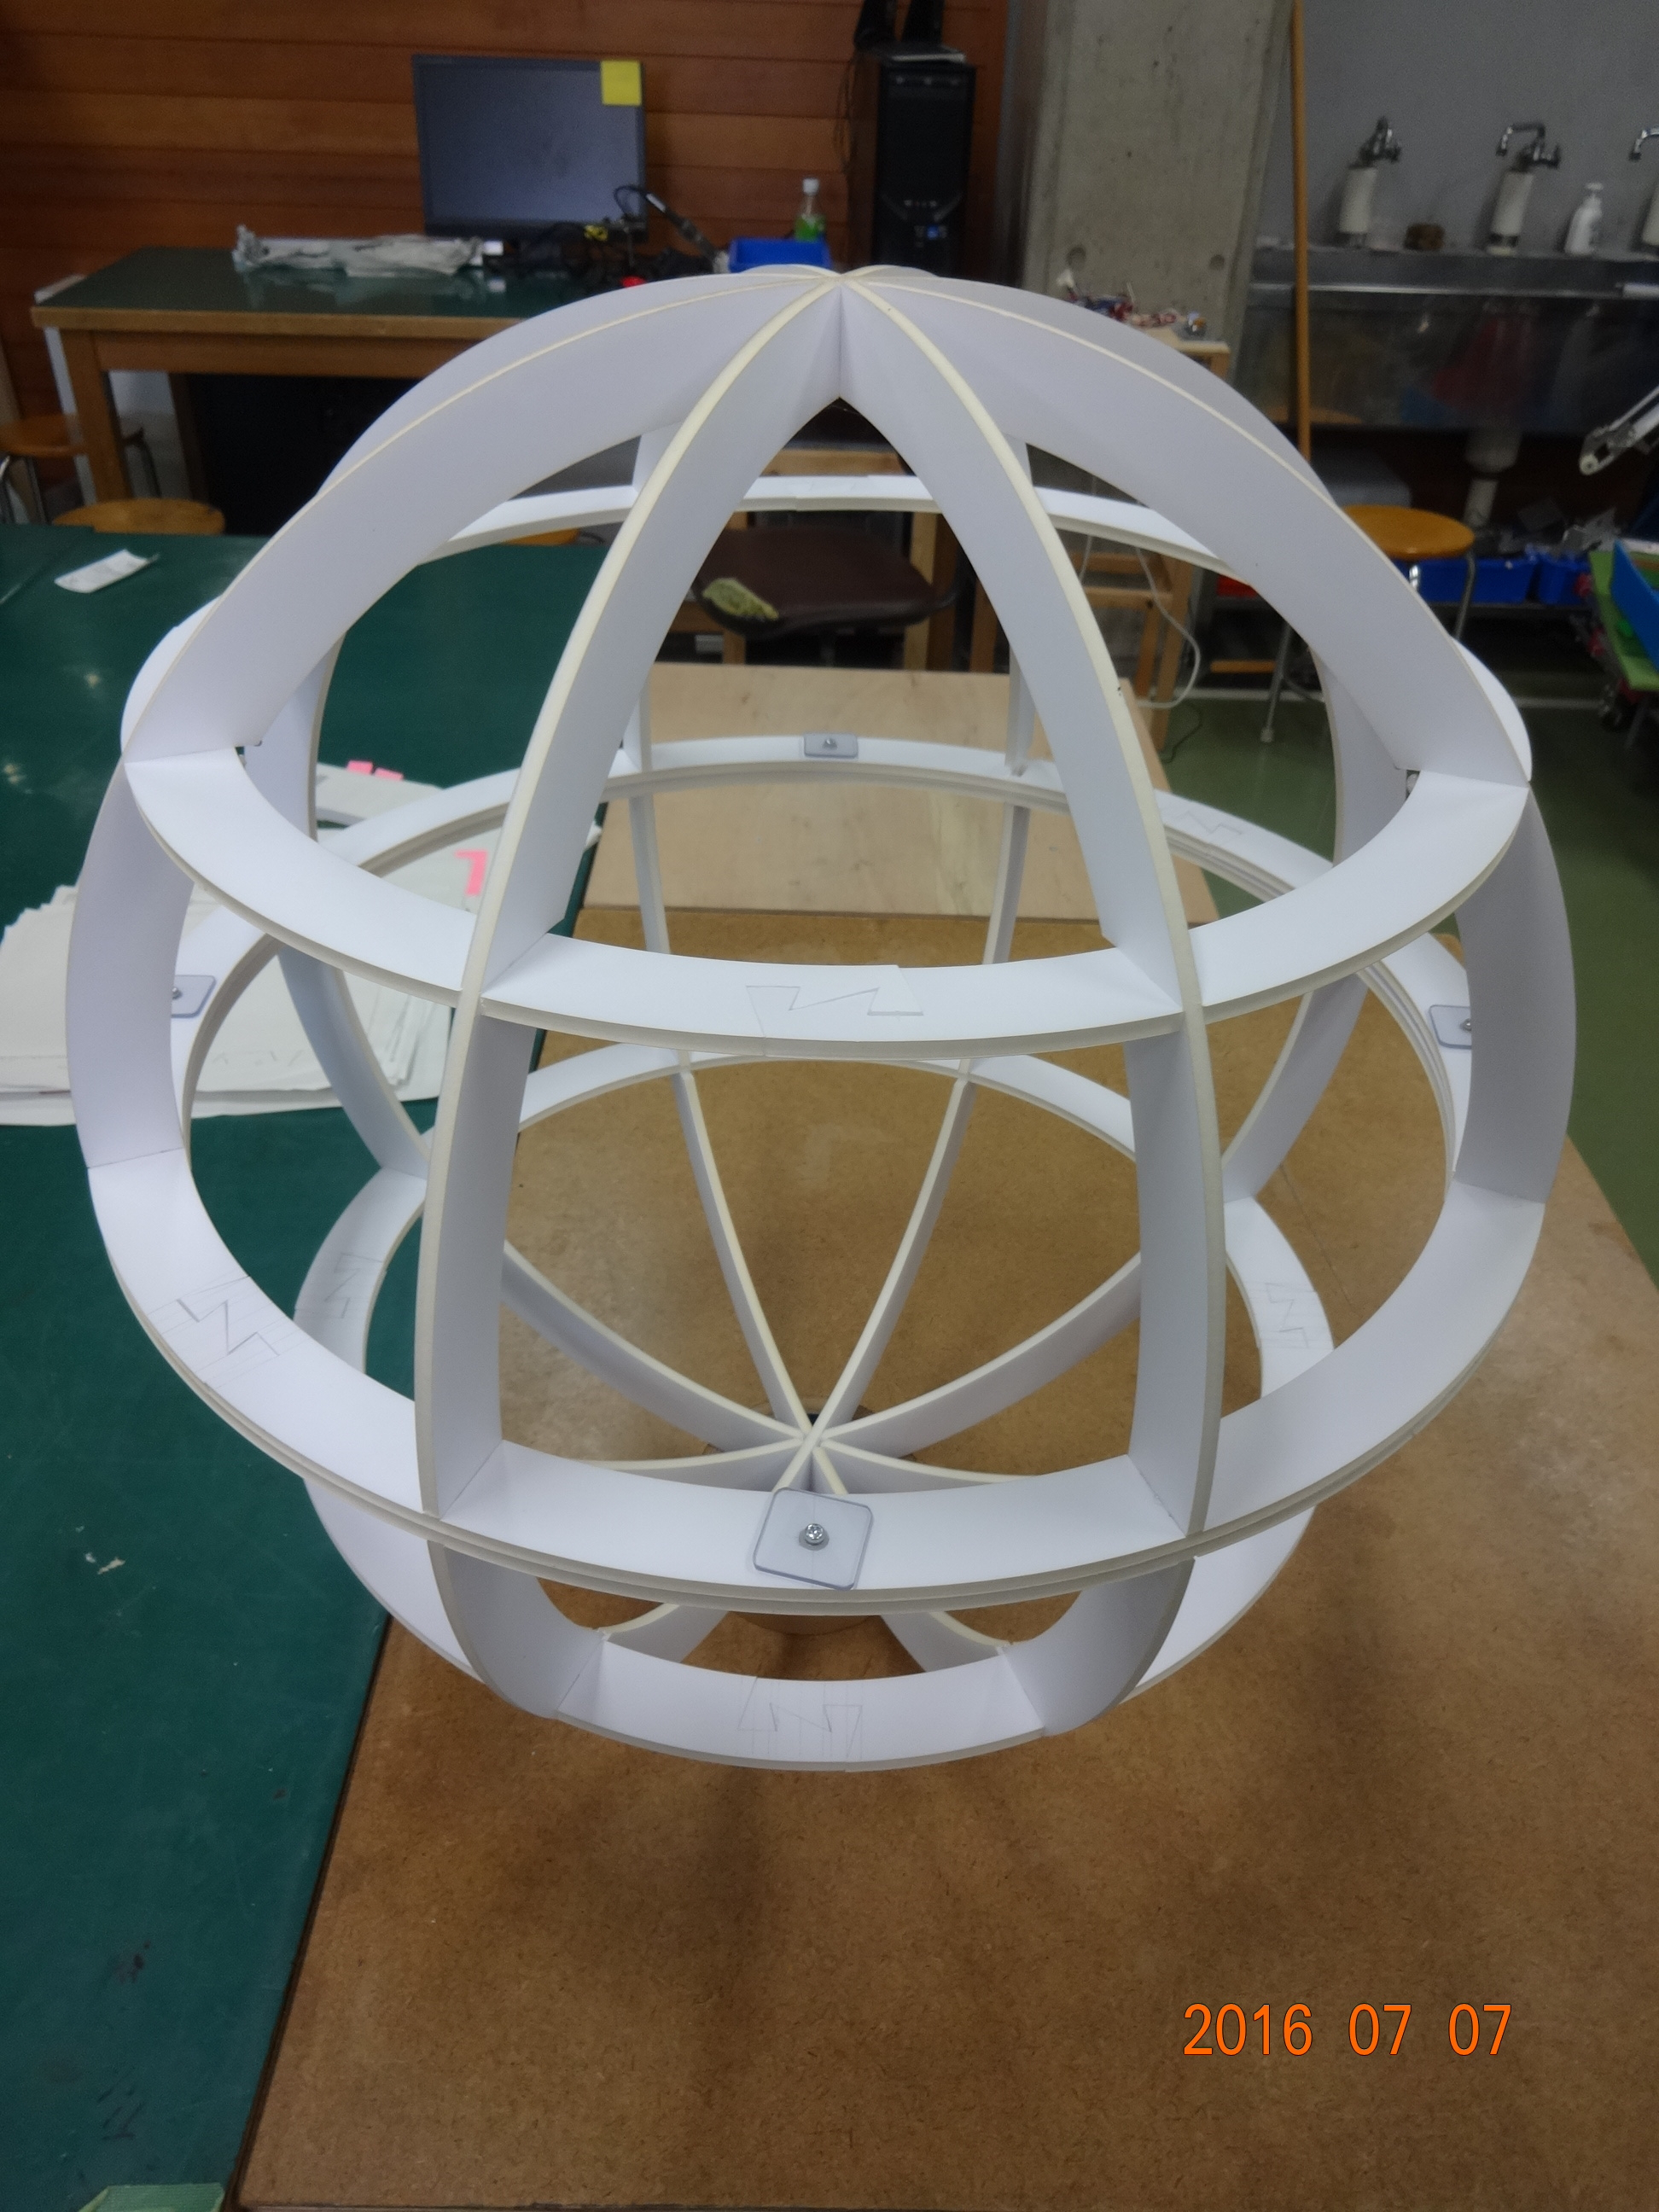
\includegraphics[width=50mm]{image/sphere-3.JPG}
  \caption{球体3号機}
  \label{fig:sphere-3}
 \end{center}
\end{figure*}

\begin{figure*}[b]
 \begin{center}
  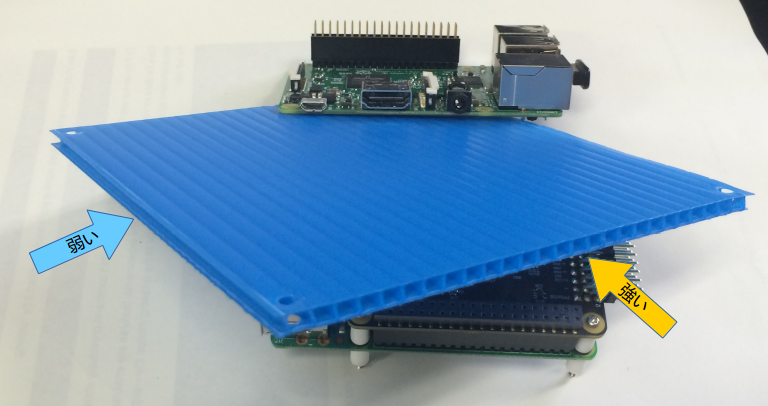
\includegraphics[width=50mm]{image/cardboard.png}
  \caption{プラスチックダンボールの特性}
  \label{fig:cardboard}
 \end{center}
\end{figure*}

%\begin{figure*}[b]
 %\begin{center}
  %\includegraphics[width=50mm]{image/sphere-4.JPG}
  %\caption{球体4号機}
  %\label{fig:sphere-4}
 %\end{center}
%\end{figure*}

\begin{figure*}[b]
 \begin{center}
  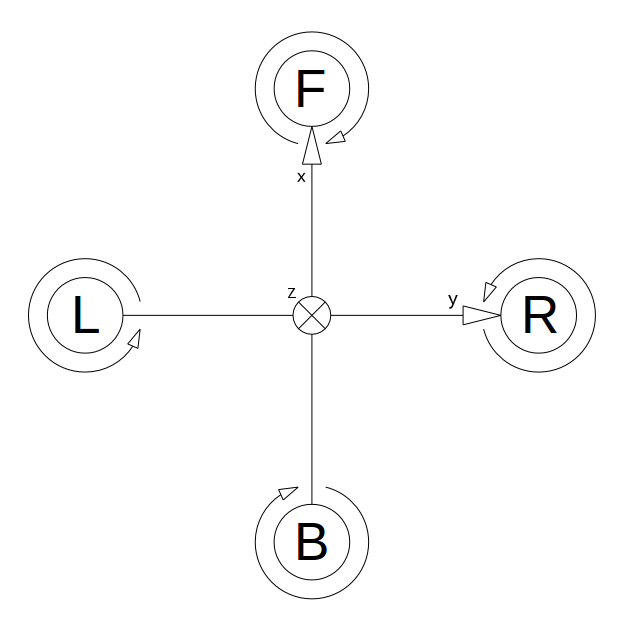
\includegraphics[width=50mm]{image/dronemotor.png}
  \caption{ドローンの座標系とモーターの回転方向}
  \label{fig:dronemotor}
 \end{center}
\end{figure*}

%%%%%%%%%%%%%%%%%%%%%%%%%%%%%%%%%%%%%%%%%%%%%%%%%%%%%%%%%%%%%%%%%%%%%%%%%%%%%%%%


\end{document}
